%%%%%%%%%%%%%%%%%%%%%%%%%%%%%%%%%%%%%%%%%%%%%%%%%%%%%%%%%%%%%%%
%
% Welcome to Overleaf --- just edit your LaTeX on the left,
% and we'll compile it for you on the right. If you open the
% 'Share' menu, you can invite other users to edit at the same
% time. See www.overleaf.com/learn for more info. Enjoy!
%
%%%%%%%%%%%%%%%%%%%%%%%%%%%%%%%%%%%%%%%%%%%%%%%%%%%%%%%%%%%%%%%
%test string
\documentclass[12pt, letterpaper]{article}
\usepackage[T1,T2A]{fontenc}     % форматы шрифтов
\usepackage[utf8x]{inputenc}     % кодировка символов, используемая в данном файле
\usepackage{colortbl}
\usepackage[russian]{babel}      % пакет русификации
\usepackage{tikz}                % для создания иллюстраций
\usepackage{pgfplots}            % для вывода графиков функций
\usepackage{geometry}		     % для настройки размера полей
\usepackage{indentfirst}         % для отступа в первом абзаце секции
\usepackage{alltt}
\usepackage{graphicx}
\usepackage{multirow}
\usepackage{hhline}
\usepackage{caption}
\usepackage{graphicx}
\usepackage{tabularx}
\usepackage{ctable} % for \specialrule command
\usepackage{tabulary}
\usepackage{amsmath}
\usepackage{epigraph}
\title{ASMbook}
\author{Анна Лыфенко\\ ВМК МГУ}
\date{Июль 2024}
\begin{document}
\maketitle
\thispagestyle{empty}
\newpage
\thispagestyle{empty}
\tableofcontents
\thispagestyle{empty}
\newpage
\section*{Введение}
\addcontentsline{toc}{section}{\protect\numberline{}Введение}
\epigraph{\textit{"Дорогу осилит идущий"}}{\textit{Луций Анней Сенека}}
Это сборник создан студентом 101 группы 1-го потока ВМК МГУ летом 2024 года для других студентов-первокурсников и не является учебным пособием! ASMbook не проходил профессиональной редактуры и может содержать ошибки и опечатки! Но всё же автор надеется, что данное творение будет полезно и поможет при подготовке к экзамену по предмету "Архитектура ЭВМ и язык ассемблера".\\
\indentВ данном сборнике приведены примеры наиболее часто встречающихся на экзамене задач (самоотверженно добытых многими поколениями ВМКшников) и решений к ним.\\
\indentПервая задача каждого раздела содержит теоретический минимум, необходимый для лучшего понимания темы. Автор настоятельно рекомендует не пропускать эти пункты. Теория позволит не просто решать заранее известные задачи, но также импровизировать при возникновении новых вопросов по старой теме.\\
\indentПервая тема "Компиляция в ассемблер" может быть полезна не только на экзамене, но и в течении семестра при сдаче контестов. Далее, разделы идут в соответствии с частотой их появления на экзамене. 1-6 темы встречались на всех экзаменах начиная с 2016 года. Вероятность их появления на Вашем экзамене довольно высока. 7 и 8 разделы встречаются реже, но тоже довольно часто.\\
\indentНемного о структуре самого экзамена.\\
Экзамен проводится на компьютере, но для решения задач он по большей части не нужен. \\
Несколько первых заданий (1-3) обычно даются на понимание языка ассемблера и во многом совпадают с заданиями коллоквиума. Для их решения достаточно знаний полученных на семинарах и при решении домашних контестов, поэтому автор не акцентирует на них внимание.\\
Далее, идут от 5 до 6 задач на темы, разобранные в данном сборнике.\\
Помимо этого есть несколько тестовых вопросов на знание материала лекций.\\
Всего 10 заданий.\\
\indentУдачи всем, сдающим предмет "Архитектура ЭВМ и язык ассемблера"!\\

Почта для обратной связи: lyfenko2006@mail.ru
\newpage
\section{Компиляция в ассемблер}
\subsection{Задача 1}
Пусть в программе на языке Си определены глобальные переменные:
\begin{verbatim}
    int *p;
    short *q;
\end{verbatim}
Приведите код на языке ассемблера, соответствующий следующему коду на языке Си:
\begin{verbatim}
    p && q && (p[2] += *q--);
\end{verbatim}
Значение вычисляемого булевого выражения после выполнения оператора должно оказаться в регистре EAX.\\
Считайте, что переменные p и q уже определены заранее, секцию данных описывать не нужно. Вам нужно реализовать только фрагмент содержимого секции .text, соответствующий фрагменту данного Си-кода.\\
\subsubsection{Теормин.}
Данная задача имеет \textbf{2 способа} решения.\\

\textbf{Первый} \textbf{способ} (ожидаемый преподавателями) — вручную переписать Си-код в ассемблер, соблюдая приоритет операций (его можно найти в интернете) и ленивую логику.\\

\textbf{Ленивая логика} — принцип вычисления булевого выражения, при котором выражение вычисляет не полностью, а до того момента, когда результат будет определен однозначно.\\

\textit{Например:}
\begin{verbatim}
    p && ((q / p) || z)
\end{verbatim}
\textit{компилятор выполнит таким образом:\\
1. Если p = 0, то возвращаем 0, ((q / p) || z) не выполняем! (потому что результат уже известен, это 0)\\
2. Если p = 1, то проверим ((q / p) || z)\\
3. Если (q / p) != 0, то z - не проверяем! (так как результат уже известен, это 1)\\
4. Если (q / p) = 0, то проверим z. Результат будет зависеть от z.\\
Поэтому, например, запись (q / p) не вернет ошибку деления на 0, т.к. если $p = 0$, мы не будем выполнять (q / p).}\\

\textbf{Второй способ}\footnote{Найден и доработан Артемом Тимофеевым} (стоит предупредить, что официально он запрещен на экзамене и при решении контестов!) — скомпилировать Си-код напрямую в ассемблер. Этот способ может быть полезен не только на экзамене, но и при решении домашних контестов. Такой метод требует большой осторожности, так как скомпилировать можно только работающую программу, а в условии требуется реализовать фрагмент кода. Следовательно, нужно не забыть удалить лишнюю часть программы.\\

\textit{Заметим! Для того чтобы редактировать скомпилированную программу, нужно хорошо разбираться в полученном коде. Рекомендуется несколько раз потренироваться, прежде чем использовать этот способ на экзамене.}\\

\textbf{Принцип работы компилятора gcc:}
\begin{figure}[h]
    \centering
    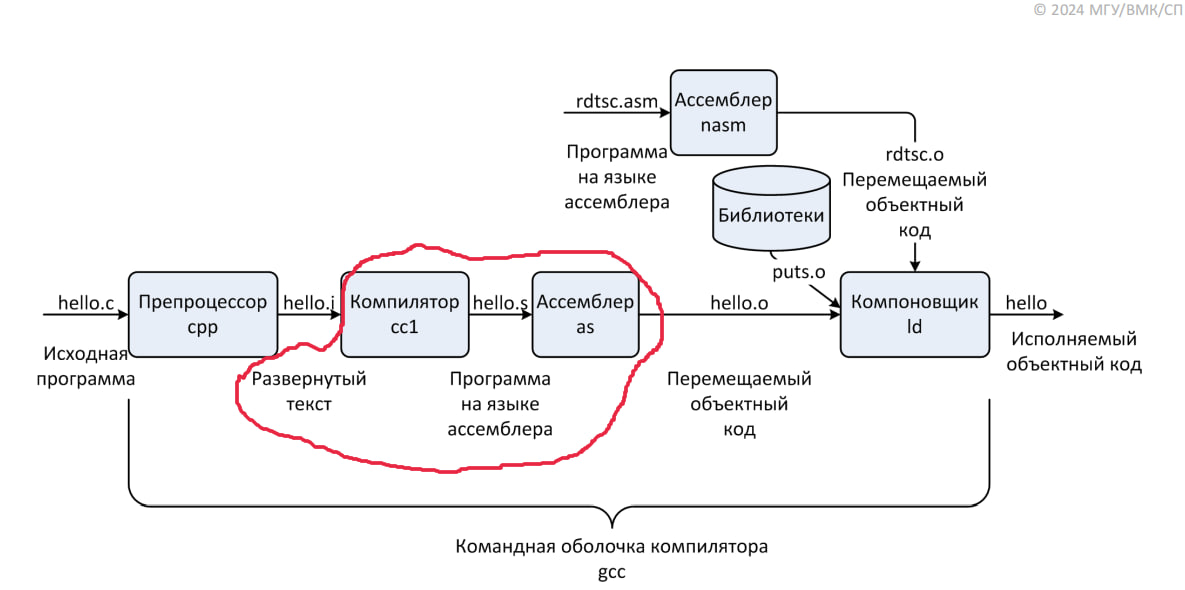
\includegraphics[width=1.0\linewidth]{image3.png}
\end{figure}\\
Нас интересует только выделенный на рисунке момент. Это компиляция Си-кода в ассемблер. Она происходит до компоновки, поэтому в ассемблерном коде мало лишней для нас информации (например нет библиотечных функций и дополнительной служебной информации, которые могут появиться, если мы возьмемся, к примеру, дизассемблировать объектный файл).\\

\textbf{Команда для компиляции в ассемблер:}\\

\textbf{gcc -S -m32 -fno-PIC -masm=intel file.c}\\

\noindentгде, gcc - компилятор\\
-S - компиляция в ассемблер\\
-m32 - ассемблер для 32-битного процессора\\
-fno-PIC - позиционно не зависимый код\\
-masm=intel - выбор нужно диалекта ассемблера\\
file.c - исходный си-файл.\\
\subsubsection{Решение}
\textbf{1 способ:}
\begin{verbatim}
    int *p;
    short *q;
\end{verbatim}
\begin{verbatim}
    p && q && (p[2] += *q--);
\end{verbatim}
Раскроем выражение: 
\begin{verbatim}
    (p[2] += *q--) = (p[2] = p[2] + *(q--))
\end{verbatim}
Приведем вручную написанный код с комментариями:
\begin{verbatim}
    xor eax, eax            ;очистили eax
    cmp dword[p], 0         ;если p = 0, то возвращаем 0 (ленивая логика)
    je .end
    cmp dword[q], 0         ;если  q = 0, то возвращаем 0 (ленивая логика)
    je .end
    mov ebx, dword[q]
    movsx ebx, word[ebx]    ;разыменовали указатель q
    sub dword[q], 2         ;уменьшили значение указателя на 2,тип short
    mov ecx, dword[p]       ;ecx = указатель на p[0]
    add ecx, 8              ;ecx = указатель на p[2], т.к. тип int
    add dword[ecx], ebx     ;p[2] += *q--
    jz .end                 ;проверили выражение на равенство 0
    inc eax                 ;если все выражения вернули 1, то результат 1
    .end:
\end{verbatim}
\textbf{2 способ:}\\
1. Запустите ОС ubuntu или виртуальную машину ubuntu.\\
2. Создайте Си-файл task1.c согласно условию задачи.\\
3. Объявите все глобальные переменные как static. Так скомпилированный файл будет более похож на написанный вручную.\\
Вот что должно получиться:
\begin{verbatim}
    #include <stdio.h>
    static int* p;
    static short *q;
    int main(void)
    {
        p && q && (p[2] += *q--);
    }
\end{verbatim}
4. Используйте команду:
\begin{figure}[h]
    \centering
    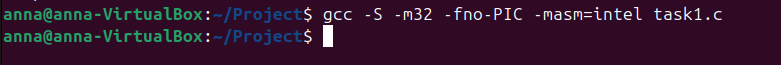
\includegraphics[width=0.75\linewidth]{image4.png}
\end{figure}\\
5. Получили ассемблерный файл task1.s.\\
6. Откройте полученный файл в SASM или текстовом редакторе.\\
Вот как он выглядит:\\
\textcolor{red}{
    .file	"task1.c"\\
	\indent .intel\_syntax noprefix\\
	\indent .text\\
	\indent .local	p\\
	\indent .comm	p,4,4\\
	\indent .local	q\\
	\indent .comm	q,4,4\\
	\indent .globl	main\\
	\indent .type	main, @function\\
main:\\
.LFB0:\\
	\indent .cfi\_startproc\\
	\indent push	ebp\\
	\indent .cfi\_def\_cfa\_offset 8\\
	\indent .cfi\_offset 5, -8\\
	\indent mov	ebp, esp\\
	\indent .cfi\_def\_cfa\_register 5}\\
	\indent mov	eax, DWORD PTR p\\
	\indent test	eax, eax\\
	\indent je	.L3\\
	\indent mov	eax, DWORD PTR q\\
	\indent test	eax, eax\\
	\indent je	.L3\\
	\indent mov	eax, DWORD PTR q\\
	\indent lea	edx, [eax-2]\\
	\indent mov	DWORD PTR q, edx\\
	\indent movzx	eax, WORD PTR [eax]\\
	\indent mov	edx, DWORD PTR p\\
	\indent add	edx, 8\\
	\indent mov	ecx, DWORD PTR [edx]\\
	\indent movsx	edx, ax\\
	\indent mov	eax, DWORD PTR p\\
	\indent add	eax, 8\\
	\indent add	edx, ecx\\
	\indent mov	DWORD PTR [eax], edx\\
	\indent mov	eax, DWORD PTR [eax]\\
	\indent test	eax, eax\\
.L3:\\
\textcolor{red}{
	\indent mov	eax, 0\\
	\indent pop	ebp\\
	\indent .cfi\_restore 5\\
	\indent .cfi\_def\_cfa 4, 4\\
	\indent ret\\
	\indent .cfi\_endproc\\
.LFE0:\\
	\indent .size	main, .-main\\
	\indent .ident	"GCC: (Ubuntu 13.2.0-23ubuntu4) 13.2.0"\\
	\indent .section	.note.GNU-stack,"",@progbits}\\
 7. Удалите все, что помечено красным.\\
 8. DWORD PTR замените на dword, аналогично с WORD PTR и т.д. Используйте для этого поиск по документу с заменой (Ctrl + f). Не забудьте добавить скобки dword[p], а не dword p.\\
 9. Рекомендую также поменять названия меток, для того, чтобы они выглядели более естественно. Например, заменить .L3 на .end.
 \begin{verbatim}
    mov	eax, dword[p]
    test	eax, eax
    je	.end
    mov	eax, dword[q]
    test	eax, eax
    je	.end
    mov	eax, dword[q]
    lea	edx, [eax-2]
    mov	dword [q], edx
    movzx	eax, word[eax]
    mov	edx, dword [p]
    add	edx, 8
    mov	ecx, dword [edx]
    movsx	edx, ax
    mov	eax, dword [p]
    add	eax, 8
    add	edx, ecx
    mov	dword [eax], edx
    mov	eax, dword [eax]
    test	eax, eax
.end:
 \end{verbatim}
 10. В данном случае значение выражения нигде не сохраняется, а по условию должно находиться в регистре eax. Поэтому нужно изменить концовку:
 \begin{verbatim}
    test	eax, eax
    je	.end
    mov eax, 1
    jmp .skip
.end:
    mov eax, 0
.skip:
 \end{verbatim}
 
 В итоге получили 2 разных решения одной задачи. 1 способ выглядит проще и быстрее, но требует знания приоритетов операции и ленивой логики. Для 2 способа нужны время и аккуратность. При этом его хорошо использовать для проверки первого способа.\\
 
 Компиляцию из си в ассемблер применима и в решении более сложных задач, при этом надо помнить, что иногда написать код вручную будет быстрее и эффективнее.\\
 
 Команду для компиляции можно менять по своему вкусу, например добавлять оптимизацию -O1 и т.д.\\
 
 P.S. Не забывайте, что компиляция из Си в ассемблер не совсем честное решение задачи, и преподаватели будут пытаться поймать Вас на незнании написанного кода.
 \newpage
 \subsection{Задача 2}
 Приведем важный пример компиляции функций с разными соглашениями вызова.\\
 
\noindent\textbf{Соглашение вызова функции:}\\
\indent cdecl - аргументы функции передаются на стеке в обратном порядке. Вызывающая функция сама убирает аргументы после выполнения вызываемой функции.\\
\indent fastcall - первые два аргумента передаются в регистрах ecx, edx соответственно. Остальные на стеке аналогично cdecl. Вызываемая функция сама убирает аргументы со стека (например, при помощи конструкции ret 0x4 - вернуться и стереть 4 верхних байта со стека, т.е. add esp, 4).\\
\indent stdcall - аргументы передаются на стеке в обратном порядке, так же как в cdecl, но стек очищается вызываемой функцией так же как в fastcall.\\

 Дан код на языке C:
 \begin{verbatim}
    #include <stdio.h>
    int f(int x) {
        return x;
    }
    int main() {
        printf("%d\n", f(4));
    }
\end{verbatim}
Необходимо перевести его в ассемблерный код, используя для функции f соглашение fastcall.
\newpage
\subsubsection{Решение}
Для начала нам потребуется изменить C-код, а именно, добавить к функции f атрибут fastcall\footnote{Можно добавить любое другое соглашение вызова}:
\begin{verbatim}
    #include <stdio.h>
\end{verbatim}
    \textcolor{orange}{\indent \_\_attribute\_\_((fastcall))} int f(int x) \{
\begin{verbatim}
        return x;
    }
    int main() {
        printf("%d\n", f(4));
    }
\end{verbatim}
Выделенная оранжевым строка сообщает компилятору, что нам необходимо скомпилировать функцию с определенным соглашением. После компиляции командой: \textbf{gcc -S -m32 -fno-PIC -masm=intel file.c} получаем:\\
\textcolor{red}{
        \indent .file	``fastcall.c''\\
	\indent .intel\_syntax noprefix\\
	\indent .text\\
	\indent .globl	f\\
	\indent .type	f, @function}\\
f:\\
\textcolor{red}{
.LFB0:\\
	\indent .cfi\_startproc}\\
	\indent push	ebp\\
\textcolor{red}{
	\indent .cfi\_def\_cfa\_offset 8\\
	\indent .cfi\_offset 5, -8}\\
	\indent mov	ebp, esp\\
\textcolor{red}{
	\indent .cfi\_def\_cfa\_register 5}\\
	\indent sub	esp, 4\\
	\indent mov	DWORD PTR [ebp-4], ecx\\
	\indent mov	eax, DWORD PTR [ebp-4]\\
	\indent leave\\
\textcolor{red}{
	\indent .cfi\_restore 5\\
	\indent .cfi\_def\_cfa 4, 4}\\
	\indent ret\\
\textcolor{red}{
	\indent .cfi\_endproc}\\
\textcolor{red}{
.LFE0:\\
	\indent .size	f, .-f}\\
	\indent .section	.rodata\\
\textcolor{red}{
.LC0:}
	\indent .string	"\%d\textbackslash n"\\
	\indent .text\\
	\indent .globl	main\\
\textcolor{red}{
        \indent .type	main, @function}\\
main:\\
\textcolor{red}{
.LFB1:\\
	\indent .cfi\_startproc}\\
	\indent lea	ecx, [esp+4]\\
\textcolor{red}{
	\indent .cfi\_def\_cfa 1, 0}\\
	\indent and	esp, -16\\
	\indent push	DWORD PTR [ecx-4]\\
	\indent push	ebp\\
	\indent mov	ebp, esp\\
\textcolor{red}{
	\indent .cfi\_escape 0x10,0x5,0x2,0x75,0}\\
	\indent push	ecx\\
\textcolor{red}{
	\indent .cfi\_escape 0xf,0x3,0x75,0x7c,0x6}\\
	\indent sub	esp, 4\\
	\indent mov	ecx, 4\\
	\indent call	f\\
	\indent sub	esp, 8\\
	\indent push	eax\\
	\indent push	OFFSET FLAT:.LC0\\
	\indent call	printf\\
	\indent add	esp, 16\\
	\indent mov	eax, 0\\
	\indent mov	ecx, DWORD PTR [ebp-4]\\
\textcolor{red}{
	\indent .cfi\_def\_cfa 1, 0}\\
	\indent leave\\
\textcolor{red}{
	\indent .cfi\_restore 5}\\
	\indent lea	esp, [ecx-4]\\
\textcolor{red}{
	\indent .cfi\_def\_cfa 4, 4}\\
	\indent ret\\
\textcolor{red}{
	\indent .cfi\_endproc\\
.LFE1:\\
	\indent .size	main, .-main\\
	\indent .ident	``GCC: (Ubuntu 13.1.0-8ubuntu1\~22.04) 13.1.0''\\
	\indent .section	.note.GNU-stack,"",\@progbits}\\
    
После редактирования получаем код в более привычном формате:\\
\begin{minipage}{0.5\textwidth}
\setlength{\parindent}{1pc}
\noindent section .rodata\\
    \indent s\_out db `\%d`,10, 0\\
section .text\\
extern printf\\
global	f\\
f:\\
    \indent push	ebp\\
    \indent mov	ebp, esp\\
    \indent sub	esp, 4\\
    \indent \textcolor{orange}{mov	dword[ebp-4], ecx}\\
    \indent mov	eax, dword [ebp-4]\\
    \indent leave\\
    \indent ret\\
global	main\\
main:\\
    \indent lea	ecx, [esp+4]\\
    \indent and	esp, -16\\
    \indent push	dword[ecx-4]\\
    \indent push	ebp\\
    \indent mov	ebp, esp\\
    \indent push	ecx\\
    \indent sub	esp, 4\\
    \indent \textcolor{orange}{mov	ecx, 4}\\
    \indent call	f\\
    \indent sub	esp, 8\\
    \indent push	eax\\
    \indent push	s\_out\\
    \indent call	printf\\
    \indent add	esp, 16\\
    \indent mov	eax, 0\\
    \indent mov	ecx, dword[ebp-4]\\
    \indent leave\\
    \indent lea	esp, [ecx-4]\\
    \indent ret\\
\end{minipage}
\begin{minipage}{0.5\textwidth}
    Обратите внимание на выделенный строки, аргумент функции передается в ecx, что характерно для fastcall.
\end{minipage}
\newpage
\section{Стек (Stack Frame)}
\subsection{Задача 1}
Дана функция на языке C:
\begin{verbatim}
    int garply(int a, int b, int c) {
        int x, y;
        scanf("%d %d", &x, &y);
        y += c ? b << a : b + x;
        return y;
    }
\end{verbatim}

Для этой функции компилятор построил следующий код:
\begin{verbatim}
    garply:
        push   esi
        push   ebx
        mov    esi, ecx
        mov    ebx, edx
        sub    esp, 0x18
    
        mov    eax, dword[gs:0x14]
        mov    dword[esp + 0x10], eax
    
        xor    eax, eax
        lea    eax, [esp + 0xc]
        push   eax
        lea    eax, [esp + 0xc]
        push   eax
        push   str
        call   scanf
        add    esp, 0x10
    
        mov    eax, dword[esp + 0x20]
        test   eax, eax
        jne    .L1
        add    ebx, dword[esp + 0x4]
    
    .L3:
        mov    eax, dword[esp + 0x8]
        add    eax, ebx
    
        mov    edx, dword[esp + 0xc]
        xor    edx, dword[gs:0x14]
        jne    .L2
    
        add    esp, 0x14
        pop    ebx
        pop    esi
        ret    0x4
    
    .L1:
        mov    ecx, esi
        shl    ebx, cl
        jmp    .L3
    
    .L2:
        call __stack_chk_fail
\end{verbatim}
В \textbf{первой строке} ответа укажите использованное при вызове данной функции соглашение вызова. Для этого выпишите \textbf{одну букву}, соответствующую верному варианту.\\
A. cdecl\\
B. fastcall\\
C. stdcall\\
D. системный вызов\\

Во \textbf{второй строке} ответа напишите цифру 1, если использовался указатель фрейма, и цифру 0 в противном случае.\\

В \textbf{третьей строке} ответа необходимо выписать состояние фрейма функции в момент времени непосредственно перед вызовом функции scanf. Требуется выписать значения ячеек памяти, начиная с адреса, по которому расположены аргументы функции garply, и заканчивая ячейкой, на которую указывает регистр ESP. Для формирования ответа выберите верные значения из списка ниже и выпишите их номера в правильном порядке в одну строку через пробел. Начинайте выписывать со значений, соответствующих \textbf{старшим} адресам ячеек памяти, и продолжайте в направлении младших адресов (т. е. в направлении роста стека). Значения могут повторяться. В скобках указан размер значений в байтах. Для последовательности выравнивающих байт размер не уточняется, т.е. любое ненулевое количество подряд идущих выравнивающих байт может быть описано единственным числом 9. Выравнивающие байты в начале ответа (если они есть) можно не выписывать.\\

\textbf{Пример форматированного ответа:}\\
A\\
0\\
16 6 1 11\\
\begin{center}
    \resizebox{\textwidth}{!}{%
    \begin{tabular}{|l|l||l|l||l|l||l|l||l|l|}
        \hline
         1 & параметр a(4)&6& колибри(4)&11&сохраненный EAX(4)&16&сохраненный ESI(4)&21&переменная x(4)\\
         \hline
         2 & параметр b(4)&7& канарейка(4)&12&сохраненный EBX(4)&17&сохраненный EDI(4)&22&переменная y(4)\\
         \hline
         3 & параметр с(4)&8& вьюрок(4)&13&сохраненный ECX(4)&18&сохраненный EBP(4)&23&адрес x(4)\\
         \hline
         4 & форматная строка(6)&9& выравнивающие байты(*)&14&сохраненный EDX(4)&19&сохраненный ESP(4)&24&адрес y(4)\\
         \hline
         5 &адрес форматной строки(4)&10& адрес возврата(4)&15&сохраненный EFX(4)&20&сохраненный EIP(4)&&\\
        \hline
    \end{tabular}}
\end{center}
\vspace{2cm}
\subsubsection{Теормин.}
В начале разберемся с тем как устроен стек.\\
Стек — это удобное для программиста представление памяти. Вместо стандартной записи памяти ``в линию'', она записывается ``в столбик''. Для того чтобы понять, какой адрес имеет не только каждая 4-байтовая ячейка стека, но и произвольный байт внутри этой ячейки, вытянем стек в линию.\\
\par
\resizebox{\textwidth}{!}{
\begin{tabular}{||l|l|l|l||l}
    \cline{1-4}
    \multicolumn{4}{||c||}{\dots} &\\
    \cline{1-4}
    \cellcolor{teal!=30} 16 & \cellcolor{teal!=30} 17 &\cellcolor{teal!=30} 18 &\cellcolor{teal!=30} 19 &\\
    \cline{1-4}
    \cellcolor{orange!=30} 12 &\cellcolor{orange!=30} 13 &\cellcolor{orange!=30} 14 &\cellcolor{orange!=30} 15 & \\
    \cline{1-4}
    \cellcolor{green!=30} 8 &\cellcolor{green!=30} 9 &\cellcolor{green!=30} 10 &\cellcolor{green!=30} 11 & $\Rightarrow$ \\
    \cline{1-4}
    \cellcolor{blue!=30} 4 &\cellcolor{blue!=30} 5 &\cellcolor{blue!=30} 6 &\cellcolor{blue!=30} 7 & \\
    \cline{1-4}
    \cellcolor{red!=30} 0 &\cellcolor{red!=30} 1 &\cellcolor{red!=30} 2 &\cellcolor{red!=30} 3 & \\
    \cline{1-4}
\end{tabular}
\begin{tabular}{||l|l|l|l||l|l|l|l||l|l|l|l||l|l|l|l||l|l|l|l||l|l|l|l||}
    \hline
    \cellcolor{red!=30}0 &\cellcolor{red!=30} 1 &\cellcolor{red!=30} 2 &\cellcolor{red!=30} 3 &\cellcolor{blue!=30} 4 &\cellcolor{blue!=30} 5 &\cellcolor{blue!=30} 6 &\cellcolor{blue!=30} 7 &\cellcolor{green!=30} 8 &\cellcolor{green!=30} 9 &\cellcolor{green!=30} 10 &\cellcolor{green!=30} 11 &\cellcolor{orange!=30} 12 &\cellcolor{orange!=30} 13 &\cellcolor{orange!=30} 14 &\cellcolor{orange!=30} 15 &\cellcolor{teal!=30} 16 &\cellcolor{teal!=30} 17 &\cellcolor{teal!=30} 18 &\cellcolor{teal!=30} 19 & \multicolumn{4}{||c||}{\dots}\\
    \hline
\end{tabular}}
В данном случае в ячейках записаны адреса байт памяти. Конечно, память по адресу 0, 1 и т. д. стеку не принадлежит (помимо стека есть еще куча и т.д.). Пример иллюстрирует только порядок в котором реальные адреса байт памяти представлены в стеке. А именно, адрес верхней ячейки будет всегда больше, чем нижней. Адрес левого байта внутри ячейки будет всегда меньше, чем правого. Сам стек растет вниз, т.е. каждый новый элемент, помещенный в стек, будет ниже предыдущего, и его адрес, соответственно, будет меньше.\\

Теперь попробуем разместить данные в стеке используя указатель стека esp и указатель фрейма ebp.\\
Пусть необходимо разместить массив из 3 элементов типа short по адресу ebp$-$6.\\
\begin{verbatim}
;short a[3] = {1, 2, 3};
push ebp
mov ebp, esp
sub esp, 12
mov word[ebp - 6], 0x1
mov word[ebp - 4],  0x2
mov word[ebp - 2],  0x3
\end{verbatim}
\begin{minipage}{.4\textwidth}
    \centering
    \begin{tabular}{r||m{1em}|m{1em}|m{1em}|m{1em}||l}
        \cline{2-5}
        &\multicolumn{4}{|c||}{\dots} &\\
        \cline{2-5}
        ebp$\longrightarrow$ &\multicolumn{4}{|c||}{\cellcolor{blue!=40} ebp} &\\
        \hhline{~----~}
        ebp$-$4$\longrightarrow$ & & & & & \\
        \hhline{~----~}
        ebp$-$8$\longrightarrow$  &  &  &  \cellcolor{green!=40}   &  &  \\
        \hhline{~----~}
        esp$\longrightarrow$  & \cellcolor{red!=40} &  & &  & \\
        \hhline{~----~}
        & &  &  &  & \\
        \cline{2-5}
        &\multicolumn{4}{|c||}{\dots} &\\
        \cline{2-5}
    \end{tabular}
    \centering
    \captionof*{table}{\textit{Синим и красным отмечены байты на которые указывают ebp и esp соответственно, зеленым - байт на который указывает ebp$-$6}}
\end{minipage}%  
\begin{minipage}{.1\textwidth}
    \raggedleft
    \begin{tabular}{c}
        $\Rightarrow$\\
        \\
        \\
        \\
        \\
        \\
        
    \end{tabular}
    \centering
\end{minipage}
\begin{minipage}{.45\textwidth}
    \centering
    \begin{tabular}{r||m{1em}|m{1em}|m{1em}|m{1em}||m{1em}}
        \cline{2-5}
        &\multicolumn{4}{|c||}{\dots} &\\
        \cline{2-5}
        ebp$\longrightarrow$ &\multicolumn{4}{|c||}{ebp} &\\
        \hhline{~----~}
        ebp$-$4$\longrightarrow$ & \cellcolor{pink!=100} 02 & \cellcolor{pink!=100} 00 & \cellcolor{pink!=130} 03 & \cellcolor{pink!=130} 00 & \\
        \hhline{~----~}
        ebp$-$8$\longrightarrow$ &  &  & \cellcolor{pink!=50} 01 & \cellcolor{pink!=50} 00 & \\
        \hhline{~----~}
        esp$\longrightarrow$ & &  &  &  & \\
        \hhline{~----~}
        & &  &  &  & \\
        \cline{2-5}
        &\multicolumn{4}{|c||}{\dots} &\\
        \cline{2-5}
    \end{tabular}
    
    \captionof*{table}{\textit{Разместили элементы массива на соответствующие места в стеке. Заметим! Байты внутри каждого short развернуты, т.к. порядок little-endian}}
\end{minipage}
\newline

Размещение элементов массива идет вверх стека, в сторону увеличения адресов.\\

Вот как выглядит этот отрезок памяти, записанный в линию:\\
\resizebox{\textwidth}{!}{
\begin{tabular}{||m{1em}||m{1em}|m{1em}|m{1em}|m{1em}||m{1em}|m{1em}|m{1em}|m{1em}||m{1em}|m{1em}|m{1em}|m{1em}||m{1em}|m{1em}|m{1em}|m{1em}||m{1em}||}
    \hline
    \dots &  &  &  &  &  &  &\cellcolor{pink!=50} 01 &\cellcolor{pink!=50} 00 &\cellcolor{pink!=100} 02 &\cellcolor{pink!=100} 00 &\cellcolor{pink!=130} 03 &\cellcolor{pink!=130} 00 & \multicolumn{4}{m{6em}||}{\centering ebp} & \dots\\
    \hline
\end{tabular}}
\resizebox{\textwidth}{!}{
\begin{tabular}{m{1em} m{1em} m{1em} m{1em} m{1em} m{1em} m{1em} m{1em} m{1em} m{1em} m{1em} m{1em} m{1em} m{1em} m{1em} m{1em} m{1em} m{1em} m{1em} m{1em} m{1em} m{1em}}
    & $\uparrow$ &  &  &  &  &  & $\uparrow$ & & & & & & \multicolumn{4}{m{6em}}{$\uparrow$} & \\
\end{tabular}}
\resizebox{\textwidth}{!}{%
\begin{tabular}{m{1em} m{1em} m{1em} m{1em} m{1em} m{1em} m{1em} m{1em} m{1em} m{1em} m{1em} m{1em} m{1em} m{1em} m{1em} m{1em} m{1em} m{1em} m{1em} m{1em} m{1em} m{1em} }
    & esp &  &  &  &  &  & ebp$-$6 & & & & & & \multicolumn{4}{m{6em}}{ebp} & \\
\end{tabular}}
\newline
Так же отметим, что иногда на стеке нужно разместить переменную, причем её тип может быть не 4-байтный. В таком случае так же удобно смотреть на стек, как на линию и располагать переменную так же, как и в обычной памяти (помним про little-endian). Например:\\
\begin{minipage}{0.6\textwidth}
    \resizebox{\textwidth}{!}{
    \begin{tabular}{|l|l|}
        \hline
        Assembler:                              & C:\\
        \hline
        sub esp, 8                             &\\
        mov dword[esp $+$ 4], 0x00000000       & long long a $=$ 123456;\\
        mov dword[esp], 0x40e20100  	       & \\
        mov byte[esp $+$ 8], 0x31              & char c $=$ '1';\\
        \hline
        \end{tabular}}
        \end{minipage}
        \begin{minipage}{\textwidth}
        \begin{tabular}{l|l|l|l|l|}
        \cline{2-5}
        &\multicolumn{4}{c|}{Стек}\\
        \cline{2-5}
        &31& & &\\
        \cline{2-5}
        &00&00&00&00\\
        \cline{2-5}
        esp$\longrightarrow$ &40&e2&01&00\\
        \cline{2-5}
    \end{tabular}
\end{minipage}
\\

Теперь внимательно посмотрим на условие задачи:\\
1. Соглашение вызова функции:\\
cdecl - аргументы функции передаются на стеке в обратном порядке. Вызывающая функция сама убирает аргументы после выполнения вызываемой функции. Например:\\
\resizebox{0.7\textwidth}{!}{
\begin{tabular}{|l|l|}
    \hline
    Assembler:                              & C:\\
    \hline
    foo:                                    & int foo(int a, int b, int c)\{\\
        \dots                               & \dots\\
        ret                                 & \}\\
        &\\
    global main &\\
    main: &\\
        \dots &\\
        push dword[c]   ; сложили аргументы &\\
        push dword[b]   ; на стек в &\\
        push dword[a]   ; обратном порядке &\\
        call foo &\\
        add  esp, 12    ; убрали аргументы &\\
        \dots &\\
    \hline
\end{tabular}}

\noindent fastcall - первые два аргумента передаются в регистрах ecx, edx соответственно. Остальные на стеке аналогично cdecl. Вызываемая функция сама убирает аргументы со стека (например, при помощи конструкции ret 0x4 - вернуться и стереть 4 верхних байта со стека, т.е. add esp, 4). Например:\\
\resizebox{0.8\textwidth}{!}{
\begin{tabular}{|l|l|}
    \hline
    Assembler:                              & C:\\
    \hline
    foo:                                    & int foo(int a, int b, int c)\{\\
        \dots                               & \dots\\
        ret  0x4    ;вызываемая функция стирает аргумент & \}\\
        &\\
    global main &\\
    main: &\\
        \dots &\\
        mov  ecx, dword[a]  ;первый аргумент в регистр ecx &\\
        mov  edx, dword[b]  ;второй аргумент в регистр edx &\\
        push dword[c]   ; третий аргумент на стек &\\
        call foo &\\
        \dots &\\
    \hline
\end{tabular}}
\\

\noindent stdcall - аргументы передаются на стеке в обратном порядке, так же как в cdecl, но стек очищается вызываемой функцией так же как в fastcall. Например:\\
\resizebox{0.8\textwidth}{!}{
\begin{tabular}{|l|l|}
    \hline
    Assembler:                              & C:\\
    \hline
    foo:                                    & int foo(int a, int b, int c)\{\\
        \dots                               & \dots\\
        ret  0x4 ;вернулись и убрали аргументы   & \}\\
        &\\
    global main &\\
    main: &\\
        \dots &\\
        push dword[c]   ; сложили аргументы &\\
        push dword[b]   ; на стек в &\\
        push dword[a]   ; обратном порядке &\\
        call foo &\\
        \dots &\\
    \hline
\end{tabular}}
\\

\noindent Системный вызов — обращение программы к ядру операционной системы для выполнения какой-либо операции. Каждая функция имеет свой номер. Вызов функции выглядит как int 0x80. Номер функции передается в регистре eax. Параметры в регистрах ebx, ecx, edx, esi, edi. Подробнее в курсе ``Операционные системы''. В данной задаче системные вызовы встречаются крайне редко. Пример системного вызова:\\
\resizebox{0.6\textwidth}{!}{
\begin{tabular}{|l|l|}
    \hline
    Assembler:                              & C:\\
    \hline
    section .data                           & \#include <unistd.h>\\
    msg db ``Hello, world!''                & \#include <stdlib.h>\\
    msg\_len equ \$-msg                     & \\
                                            &void main() \{\\
    section .text                           &write(1, ``Hello, world!'', 14);\\
    global \_start                          &exit(0);\\
    \_start:                                &\}\\
    mov eax, 4                              &\\
    mov ebx, 1                              &\\
    mov ecx, msg                            &\\
    mov edx, msg\_len                       &\\
    int 80h                                 &\\
    &\\
    mov eax, 1                              &\\
    mov ebx, 0                              &\\
    int 80h                                 &\\
    \hline
\end{tabular}}
\\

2. Указатель фрейма — это регистр ebp. Указатель стека — регистр esp.\\

Иногда в данной задаче требуется указать методы защиты. Перечислим основные из них:\\
1. \textbf{Канарейка на стеке}.\\
\indentКанарейка — число, генерируемое ОС и хранящееся по адресу gs:20 (иногда пишут gs:0x14), где gs - сегментный регистр. Отключается опцией -fno-stack-protector.\\
\indent\textbf{Принцип работы:} канарейка кладется на стек в начале функции. После завершения работы функции, но до выхода из нее сохранность канарейки проверяется. Если она оказалась ``затёрта'', т.е. канарейка на стеке не совпадает с изначальным значением по адресу gs:0x14, то функция отработала не корректно, вызываем прерывание \_\_stack\_chk\_fail. Иначе все в порядке, выходим из функции.\\
\indent\textbf{Показатель присутствия} защиты ``канарейка'', строки:\\
mov eax, dword[gs:0x14]\\
call \_\_stack\_chk\_fail\\
2. \textbf{DEP}.\\
\indent Data Execution Prevention (предотвращение исполнения данных). Реализуется аппаратурой и ОС.\\
\indent \textbf{Принцип работы:} позволяет помечать область памяти ``только для данных''. Код, записанный в такую область нельзя исполнять.\\
3. \textbf{ASLR}.\\
\indent Address Space Layout Randomization (рандомизация размещения адресного пространства). Реализуется ОС.\\
\indent \textbf{Принцип работы:} основные компоненты программы (стек, код, куча и т.д.) размещаются на случайных базовых адресах.\\
4. \textbf{CFI}.\\
\indent Control Flow Integrity (целостность потока управления) - комплекс методов для передачи управления ``туда, куда надо''.\\
5. \textbf{Intel CET}\\
\indent Control-flow Enforcement Technology (Технология обеспечения контроля потока данных).\\
\indent \textbf{Принцип работы:} создание теневого стека (Shadow Stack). Перед выходом из функции адрес возврата из основного стека сверяется с адресом возврата из теневого стека. При несовпадении — аварийная остановка.\\
\indent \textbf{Показатель присутствия} защиты CET, команда:\\
ENDBR
\newpage
\subsubsection{Решение}
1. Заметим:\\
\dots\\
mov esi, ecx\\
mov ebx, edx\\
\dots\\
ret 0x4\\
\dots\\
Первые 2 аргумента переданы в регистрах, вызываемая функция сама убирает параметры со стека, значит соглашение о вызове - fastcall.\\

2. Указатель фрейма, то есть регистр ebp не используется.\\

3. Теперь изобразим стек:\\

Разберем код по частям:\\
\begin{minipage}{.4\textwidth}
    \noindent garply:\\
        push   esi\\
        push   ebx\\
        mov    esi, ecx\\
        mov    ebx, edx\\
    \dots\\
\end{minipage}%  
\begin{minipage}{.4\textwidth}
    \resizebox{1.3\textwidth}{!}{%
    \begin{tabular}{r||m{6em}||l|}
        \cline{2-3}
        &\dots & \dots\\
        \cline{2-3}
        & c & аргумент c\\
        \cline{2-3}
        & ret adr &адрес возврата\\
        \cline{2-3}
        & esi & сохраненный esi\\
        \cline{2-3}
        esp$\longrightarrow$ & ebx & сохраненный ebx\\
        \cline{2-3}
        &\dots & \dots\\
        \cline{2-3}
    \end{tabular}}
\end{minipage}% 

Далее сдвинем esp вниз на 24 (в десятичной системе) и поместим канарейку на стек:\\
\begin{minipage}{.4\textwidth}
    \dots\\
    sub    esp, 0x18\\
    mov    eax, dword[gs:0x14]\\
    mov    dword[esp + 0x10], eax\\
    \dots\\
\end{minipage}% 
\begin{minipage}{.4\textwidth}
    \resizebox{1.3\textwidth}{!}{%
    \begin{tabular}{r||m{6em}||l|}
        \cline{2-3}
        &\dots & \dots\\
        \cline{2-3}
        & c & аргумент c\\
        \cline{2-3}
        & ret adr &адрес возврата\\
        \cline{2-3}
        & esi & сохраненный esi\\
        \cline{2-3}
        & ebx & сохраненный ebx\\
        \cline{2-3}
        &       &\\
        \cline{2-3}
        & dword[gs:0x14] & канарейка\\
        \cline{2-3}
        &       &\\
        \cline{2-3}
        &       &\\
        \cline{2-3}
        &       &\\
        \cline{2-3}
        esp$\longrightarrow$ &       &\\
        \cline{2-3}
        &\dots & \dots\\
        \cline{2-3}
    \end{tabular}}
\end{minipage}%  
\\

Теперь подготовим стек к вызову функции scanf\\
\begin{minipage}{.4\textwidth}
    \dots\\
    \noindent xor    eax, eax\\
    lea    eax, [esp $+$ 0xc]\\
    push   eax\\
    lea    eax, [esp $+$ 0xc]\\
    push   eax\\
    push   str\\
    call   scanf\\
    \dots\\
\end{minipage}
\begin{minipage}{.4\textwidth}
    \resizebox{1.37\textwidth}{!}{
    \begin{tabular}{r||m{6em}||l|l}
        \cline{2-3}
        &\dots & \dots\\
        \cline{2-3}
        & c & аргумент c&\\
        \cline{2-3}
        & ret adr &адрес возврата & \cellcolor{black}\\
        \cline{2-3}
        & esi & сохраненный esi&\\
        \cline{2-3}
        & ebx & сохраненный ebx&\\
        \cline{2-3}
        &   $-$    &\\
        \cline{2-3}
        & dword[gs:0x14] & канарейка&\cellcolor{black}\\
        \cline{2-3}
        &   y   &переменная y&\\
        \cline{2-3}
        &   x   &переменная x&\\
        \cline{2-3}
        &    $-$  &\\
        \cline{2-3}
        &   $-$  & &\cellcolor{black}\\
        \cline{2-3}
        &   \&y  &адрес переменной y\\
        \cline{2-3}
        &   \&x  &адрес переменной x\\
        \cline{2-3}
        esp$\longrightarrow$ & str &адрес форматной строки\\
        \cline{2-3}
        &\dots & \dots\\
        \cline{2-3}
    \end{tabular}}
\end{minipage}%

Выравнивающие байты отмечены прочерком. Черные квадраты показывают адреса кратные 4. Теперь мы видим, что перед вызовом функции scanf стек, как и полагается, выровнен по 4. Стоит отметить, что в ассемблерном коде нет никаких переменных x и y.\\ 
\\
Команды:\\
lea eax, [esp $+$ 0xc]\\
push eax\\
кладут на стек адрес определенного места на стеке. Глядя на код С и аргументы функции scanf мы догадываемся, что указанные адреса это места расположения на стеке автоматических переменных, которые в коде на языке C названы y и x. Эти 2 команды повторены два раза. Первый раз для переменной y, второй раз для переменной x, которая на стеке располагается ниже переменной y, т.к. команда push сдвигает esp вниз на 4.\\
Проделанных действий достаточно, для того, чтобы дать ответ. Он будет выглядеть так:\\

\noindentОтвет:\\
B\\
0\\
3 10 16 12 9 7 22 21 9 24 23 5
\newpage
\subsection{Задача 2}
Дана функция на языке C:
\begin{verbatim}
    int thud(short *src, int n) {
        short m[14];
        memcpy(m, src, n);
        int x = 0;
        for(int i = 0; i < n; i++)
            x += m[i];
        return x;
    }
\end{verbatim}
Для этой функции компилятор построил следующий код\footnote{Автора удивило использование dword[\dots] и WORD PTR [edx] в одном ассемблерном коде, вероятно это опечатка и имелось ввиду word[edx].}:
\begin{verbatim}
    thud:
        push    ebp
        mov     ebp, esp
        push    ebx
        sub     esp, 0x28
        mov     ebx, dword[ebp + 0xc]
    
        mov     eax, dword[gs:0x14]
        mov     dword[ebp - 0xc], eax
        xor     eax, eax
    
        lea     eax, [ebp - 0x28]
        push    ebx
        push    dword[ebp + 0x8]
        push    eax
        call    memcpy
        add     esp, 0x10
    
        test    ebx, ebx
        jle     .L1
        lea     edx, [ebp - 0x28]
        lea     ebx, [edx + ebx * 2]
        mov     eax, 0x0
    
    .L2:
        movsx   ecx, WORD PTR [edx]
        add     eax, ecx
        add     edx, 0x2
        cmp     edx, ebx
        jne     .L2
        jmp     .L3
    
    .L1:
        mov eax, 0x0
    
    .L3:
        mov     ebx, dword[ebp - 0xc]
        xor     ebx, dword[gs:0x14]
        je      .L4
        call    __stack_chk_fail
    
    .L4:
        mov     ebx, dword[ebp - 0x4]
        leave
        ret     0x8
\end{verbatim}
В \textbf{первой строке} ответа укажите использованное при вызове данной функции соглашение вызова. Для этого выпишите \textbf{одну букву}, соответствующую верному варианту.\\
A. cdecl\\
B. fastcall\\
C. stdcall\\
D. системный вызов\\

Во \textbf{второй строке} ответа напишите цифру 1, если использовался указатель фрейма, и цифру 0 в противном случае.\\

В \textbf{третьей строке} ответа необходимо выписать состояние фрейма функции в момент времени непосредственно перед вызовом функции memcpy. Требуется выписать значения ячеек памяти, начиная с адреса, по которому расположены аргументы функции thud, и заканчивая ячейкой, на которую указывает регистр ESP. Для формирования ответа выберите верные значения из списка ниже и выпишите их номера в правильном порядке в одну строку через пробел. Начинайте выписывать со значений, соответствующих \textbf{старшим} адресам ячеек памяти, и продолжайте в направлении младших адресов (т. е. в направлении роста стека). Значения могут повторяться. В скобках указан размер значений в байтах. Для последовательности выравнивающих байт размер не уточняется, т.е. любое ненулевое количество подряд идущих выравнивающих байт может быть описано единственным числом 9. Выравнивающие байты в начале ответа (если они есть) можно не выписывать.\\

\textbf{Пример форматированного ответа:}\\
A\\
0\\
16 6 1 11\\
\begin{center}
    \resizebox{\textwidth}{!}{
    \begin{tabular}{|l|l||l|l||l|l||l|l||l|l|}
        \hline
         1 & параметр src(4)&6& колибри(4)&11&сохраненный EAX(4)&16&сохраненный ESI(4)&21&переменная i(4)\\
         \hline
         2 & параметр n(4)&7& канарейка(4)&12&сохраненный EBX(4)&17&сохраненный EDI(4)&22&адрес переменной i(4)\\
         \hline
         3 & переменная x(4)&8& вьюрок(4)&13&сохраненный ECX(4)&18&сохраненный EBP(4)\\
         \cline{1-8}
         4 & адрес массива m(4)&9& выравнивающие байты(*)&14&сохраненный EDX(4)&19&сохраненный ESP(4)\\
         \cline{1-8}
         5 &массив m(28)&10& адрес возврата(4)&15&сохраненный EFX(4)&20&сохраненный EIP(4)\\
        \cline{1-8}
    \end{tabular}}
\end{center}
\vspace{2cm}
\subsubsection{Решение}
1. Заметим:\\
\dots\\
mov ebx, dword[ebp + 0xc]\\
\dots\\
push ebx\\
push dword[ebp + 0x8]\\
\dots\\
ret 0x8\\
\dots\\
Оба аргумента переданы на стеке, вызываемая функция сама убирает параметры со стека, значит соглашение о вызове - stdcall.\\

2. Указатель фрейма, то есть регистр ebp используется.\\
push ebp\\
mov ebp, esp\\

3. Теперь изобразим стек:\\

Разберем код по частям:\\
\begin{minipage}{.4\textwidth}
    \noindent thud:\\
        push   ebp\\
        mov    ebp, esp\\
        push   ebx\\
    \dots\\
\end{minipage}  
\begin{minipage}{.4\textwidth}
    \resizebox{1.3\textwidth}{!}{%
    \begin{tabular}{r||m{6em}||l|}
        \cline{2-3}
        &\dots & \dots\\
        \cline{2-3}
        & n & параметр n\\
        \cline{2-3}
        & src & параметр src\\
        \cline{2-3}
        & ret adr & адрес возврата\\
        \cline{2-3}
        ebp$\longrightarrow$ & ebp &сохраненный ebp\\
        \cline{2-3}
        esp$\longrightarrow$ & ebx & сохраненный ebx\\
        \cline{2-3}
        &\dots & \dots\\
        \cline{2-3}
    \end{tabular}}
\end{minipage} 

Далее сдвинем esp вниз на 40 (в десятичной системе) и поместим канарейку на стек:\\
\begin{minipage}{.4\textwidth}
    \dots\\
    sub esp, 0x28\\
    mov ebx, dword[ebp + 0xc]\\
    mov eax, dword[gs:0x14]\\
    mov dword[ebp - 0xc], eax\\
    \dots\\
\end{minipage} 
\begin{minipage}{.4\textwidth}
    \resizebox{1.3\textwidth}{!}{
    \begin{tabular}{r||m{6em}||l|}
        \cline{2-3}
        &\dots & \dots\\
        \cline{2-3}
        & n & параметр n\\
        \cline{2-3}
        & src & параметр src\\
        \cline{2-3}
        & ret adr & адрес возврата\\
        \cline{2-3}
        ebp$\longrightarrow$ & ebp &сохраненный ebp\\
        \cline{2-3}
        & ebx & сохраненный ebx\\
        \cline{2-3}
        & &\\
        \cline{2-3}
        & dword[gs:0x14] & канарейка\\
        \cline{2-3}
        & &\\
        \cline{2-3}
        & &\\
        \cline{2-3}
        & &\\
        \cline{2-3}
        & &\\
        \cline{2-3}
        & &\\
        \cline{2-3}
        & &\\
        \cline{2-3}
        & &\\
        \cline{2-3}
        esp$\longrightarrow$ & &\\
        \cline{2-3}
        &\dots & \dots\\
        \cline{2-3}
    \end{tabular}}
\end{minipage} 
\\
Теперь подготовим стек к вызову функции memcpy\\
\begin{minipage}{.4\textwidth}
    \dots\\
    \noindent xor eax, eax\\
    lea eax, [ebp - 0x28]\\
    push ebx\\
    push dword[ebp + 0x8]\\
    push eax\\
    call memcpy\\
    \dots\\
\end{minipage}% 
\begin{minipage}{.4\textwidth}
    \resizebox{1.37\textwidth}{!}{%
    \begin{tabular}{r||m{3em}|m{3em}||l|l}
        \cline{2-4}
        &\multicolumn{2}{m{6em}||}{\dots}& \dots&\\
        \cline{2-4}
        &\multicolumn{2}{m{6em}||}{n} & параметр n &\\
        \cline{2-4}
        &\multicolumn{2}{m{6em}||}{src}& параметр src&\\
        \cline{2-4}
        &\multicolumn{2}{m{6em}||}{ret adr}& адрес возврата&\cellcolor{black}\\
        \cline{2-4}
        ebp$\longrightarrow$ & \multicolumn{2}{m{6em}||}{ebp}&сохраненный ebp&\\
        \cline{2-4}
        &\multicolumn{2}{m{6em}||}{ebx}& сохраненный ebx&\\
        \cline{2-4}
        & \multicolumn{2}{m{6em}||}{} & &\\
        \cline{2-4}
        & \multicolumn{2}{m{6em}||}{dword[gs:0x14]} & канарейка&\cellcolor{black}\\
        \cline{2-4}
        & m[12] & m[13] & &\\
        \cline{2-4}
        & m[10] & m[11] & &\\
        \cline{2-4}
        & m[8] & m[9] & &\\
        \cline{2-4}
        & m[6] & m[7] & &\cellcolor{black}\\
        \cline{2-4}
        & m[4] & m[5] & &\\
        \cline{2-4}
        & m[2] & m[3] & &\\
        \cline{2-4}
        & m[0] & m[1] & массив m &\\
        \cline{2-4}
        &\multicolumn{2}{m{6em}||}{-}& & \cellcolor{black}\\
        \cline{2-4}
        &\multicolumn{2}{m{6em}||}{n}& параметр n & \\
        \cline{2-4}
        &\multicolumn{2}{m{6em}||}{src}& параметр src & \\
        \cline{2-4}
        esp$\longrightarrow$ &\multicolumn{2}{m{6em}||}{\&m[0]}& адрес массива m& \\
        \cline{2-4}
        &\multicolumn{2}{m{6em}||}{\dots}& \dots &\\
        \cline{2-4}
    \end{tabular}}
\end{minipage} \\

Выравнивающие байты отмечены прочерком. Черные квадраты показывают адреса кратные 4. Теперь мы видим, что перед вызовом функции memcpy стек, как и полагается, выровнен по 4.\\ 
\noindentОтвет: C; 1; 2 1 10 18 12 9 7 5 9 2 1 4. \textbf{Формат ответа указан в условии!}
\newpage
\section{Вещественные числа (IEEE 754)}
\subsection{Задача 1}
Используется 10-битный формат, удовлетворяющий требованиям стандарта IEEE 754: знаковый бит, 4 бита — порядок, 5 битов — мантисса.\\

Выпишете:
\begin{itemize}
    \item Двоичное представление ближайшего к нулю отрицательного денормализованного, D;
    \item Модуль разности между соседними денормализованными числами в виде обыкновенной несократимой дроби, S;
    \item Двоичное представление $I=-113$ (минус сто тринадцать);
    \item Двоичное представление $F=1/12$ (одна двенадцатая);
\end{itemize}

Округление выполнять к ближайшему чётному.
\vspace{2cm}
\subsubsection{Теормин.}
\textbf{IEEE 754} - это стандарт, который описывает формат представление числа с плавающей точкой.\\
Согласно этому стандарту, любое вещественное число A представляется как:\\
\[A=(-1)^s*2^E*M\]
где s - знаковый бит, если число положительное - 0, иначе 1;\\
M - мантисса, число из промежутка [1;2) для нормализованных, или из промежутка [0,1) для денормализованных.\\
E - порядок, степень в которую нужно возвести 2, чтобы $(-1)^s*2^E*M=A$

Далее число записывается таким образом (\textbf{двоичное представление}):\\
\begin{tabular}{|c|c|c|}
    \hline
     s   &  exp  &  frac  \\
    \hline
    \multicolumn{1}{c}{\raisebox{.5\normalbaselineskip}[0pt][0pt]{$\underbrace{\phantom{bbbb бит}\hspace*{5\tabcolsep}}$}} & \multicolumn{1}{c}{\raisebox{.5\normalbaselineskip}[0pt][0pt]{$\underbrace{\phantom{bbbb бит}\hspace*{5\tabcolsep}}$}} & \multicolumn{1}{c}{\raisebox{.5\normalbaselineskip}[0pt][0pt]{$\underbrace{\phantom{bbbbbbb бит}\hspace*{5\tabcolsep}}$}}\\
    \multicolumn{1}{c}{Знаковый}&\multicolumn{1}{c}{Порядок}&\multicolumn{1}{c}{Мантисса}\\
    \multicolumn{1}{c}{бит}&\multicolumn{1}{c}{$+$}&\multicolumn{1}{c}{без}\\
    \multicolumn{1}{c}{}&\multicolumn{1}{c}{Смещение}&\multicolumn{1}{c}{целой части}\\
\end{tabular}

Поясним:\\
\textbf{Смещение} - это число равное $2^{k-1}-1$, где k - это количество бит, которыми кодируется экспонента exp.\\
\textbf{exp} - экспонента, $exp = \text{смещение} + E$, где E - это порядок.\\
\textbf{frac} - это мантисса без целой части, т.е. если мантисса 1.101, то $frac=101$.\\
\textit{Пример:}\\
\textit{Пусть под кодировку мантиссы M отдано 3 бита, а порядок E кодируется 4 битами\footnote{Здесь говорится ``мантисса'' и ``порядок'', хотя имеется ввиду frac и exp. На самом деле, frac это способ кодировки мантиссы, а exp соответственно порядка, поэтому допустимо говорить ``порядок'' и иметь в виду его кодировку exp или ``мантисса'' и иметь в виду её кодировку frac.}, как будет выглядеть число $15,25_{10}$ в кодировке IEEE 754? Округление происходит к ближайшему четному}.\\
\textit{Решение:
\[15,25_{10} = 1111.01_2 = (-1)^0 * 2^3 * 1.11101\]
Значит, $frac = 11101$, округлим до 3 цифр (т.к. под мантиссу выделено 3 бита): $frac = 111$.\\
$\text{Порядок} = 3_{10}$
$\text{Смещение} = 2^{4 - 1} - 1 = 2^3 - 1 = 7$, тогда:\\
$exp = E + \text{смещение} = 3 + 7 = 10_{10} = 1010_2$.\\
Число выглядит так:
\begin{tabular}{ccc}
    0 & 1010 & 111\\
    \multicolumn{1}{c}{\raisebox{.5\normalbaselineskip}[0pt][0pt]{$\underbrace{\phantom{т}\hspace*{5\tabcolsep}}$}} & \multicolumn{1}{c}{\raisebox{.5\normalbaselineskip}[0pt][0pt]{$\underbrace{\phantom{bбит}\hspace*{5\tabcolsep}}$}} & \multicolumn{1}{c}{\raisebox{.5\normalbaselineskip}[0pt][0pt]{$\underbrace{\phantom{bбит}\hspace*{5\tabcolsep}}$}}\\
    \multicolumn{1}{c}{s}&\multicolumn{1}{c}{exp}&\multicolumn{1}{c}{frac}\\
\end{tabular}
Ответ: 01010111.}\\

\textit{Заметим! Что представление числа в формате IEEE 754 (называемое также двоичным представлением числа) и представление числа в двоичной системе счисления, это абсолютно разные и не связанные между собой понятия.}\\

Теперь разберемся, что такое нормализованные, денормализованные и особые числа.\\

\textbf{Нормализованное число} — это число, порядок exp которого не принимает крайние значения, т.е. 00\dots0 или 11\dots1. Например, число из предыдущего примера.\\

\textbf{Денормализованное число} — это число, порядок exp которого 00\dots0. При этом значение порядка $E = 1 - \text{Смещение}$. $\text{Мантисса} = 0.xxx\dots x$, где xxx\dots x - Биты поля frac. Денормализованные числа, очевидно, близки к нулю. \\
\textit{Например:\\
Число, которое в представлении IEEE 754 выглядит так: 1 0000 010.\\
$exp = 0$, $frac = 010$.\\
$\text{Смещение} = 2^{4 - 1} - 1 = 7$\\
$E = 1 - \text{смещение} = 1 - 7 = -6$\\
$M = 0.010_2 = 0,25_{10}$, у M целая часть 0, а не 1, т.к. число денормализованное.}\\
\textit{В обычном представлении это было бы число:\\
$(-1)^1 * 2^{-6} * 0,25 = -0,00390625$.}\\

\textit{Заметим!}\\
\textit{Чем больше бит кодирует порядок, тем более близкие к нулю числа можно представить в виде нормализованных чисел.}\\
\textit{Чем больше бит кодирует мантиссу, тем более точно можно представить число.}\\

\textbf{Особое число} — это число, порядок exp которого 11\dots1. При этом, если мантисса frac = 00\dots0, то такое число $\pm\infty$ (знак зависит от бита s). Иначе, NaN (Not-a-Number). NaN используется в ситуациях, когда значение операции не определено (например после деления на 0).
\begin{figure}[h]
    \centering
    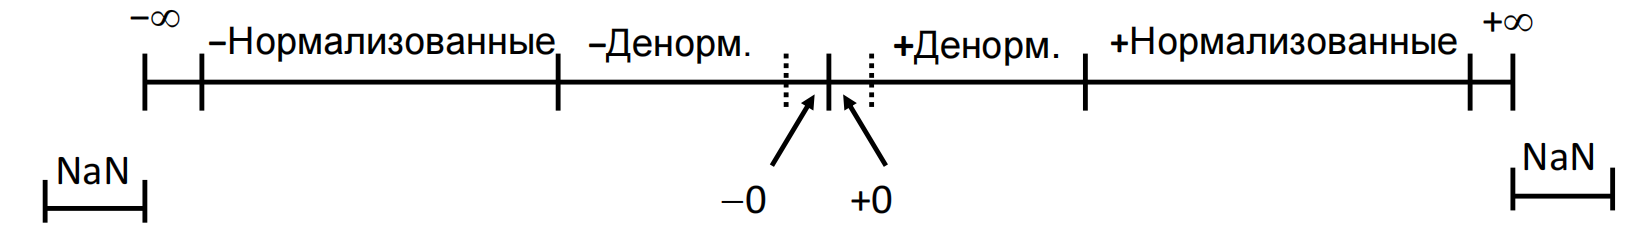
\includegraphics[width=0.75\linewidth]{image2.png}
\end{figure}

В условии возникла фраза: ``Округление выполнять к ближайшему четному''. Поэтому разберемся с \textbf{видами округления.}\\
Есть 4 основных способа округления:
\begin{itemize}
    \item к нулю
    \item к наибольшему ($+\infty$)
    \item к наименьшему ($-\infty$)
    \item к ближайшему
\end{itemize}
На деле, используется только округление \textbf{к ближайшему}, т.к. остальные способы накапливают большую погрешность.\\

Но как поступить, когда число расположено ровно посередине между двух значений, к которым нужно округлить? Здесь и возникает \textbf{округление к ближайшему четному}. Т.е. округление происходит так, чтобы последняя цифра получившегося числа была четной. Например: $13,2500\approx13,2$; $13,35\approx13,4$. Или, в двоичной системе, $101.010\approx101.0$; $101.110\approx110.0$.\\

\subsubsection{Решение}
1) Двоичное представление ближайшего к нулю отрицательного денормализованного, D;\\
$s = 1$, т.к. отрицательное.\\
$exp = 0000$, т.к. денормализованное.\\
$frac = 00001$, т.к. ближайшее к нулю.\\
Значит, двоичное представление числа: 1000000001.\\

2) Модуль разности между соседними\footnote{В математике определить ``соседние'' вещественные числа нельзя, т.к. вещественные числа вообще говоря бесконечные дроби. Но в памяти компьютера любое представление конечно, поэтому вещественных чисел, представимых в памяти компьютера, конечное количество, и их можно расположить по порядку. Например: 000001, 000010, 000011 и т.д. (формат IEEE 754).} денормализованными числами в виде
обыкновенной несократимой дроби, S;\\
0 0000 00000 - ноль, денормализованное число.\\
0 0000 00001 - ближайшее к нулю положительное денормализованное число.\\
Значит, расстояние между двумя денормализованными числами - 0 0000 00001. Осталось перевести из двоичной записи \textit{(формат IEEE 754. Не путать с записью в двоичной системе счисления!)} в десятичную.\\
$\text{Смещение} = 2^{4-1} - 1 = 7$\\
$E = 1 - \text{Смещение} = 1 - 7 = -6$\\
$M = 0.00001_2 = \frac{1}{32}_{10}$\\
Искомая разность: $(-1)^0 * 2^{-6} * \frac{1}{32} = 2^{-11} = \frac{1}{2048}$\\

3) Двоичное представление $I=-113$ (минус сто тринадцать);\\
$-113_{10} = -1110001_2 =(-1)^1 * 2^6 * 1.110001$. Значит:\\
$s = 1$\\
$E = 6$\\
$frac = 11000$, округлили к ближайшему четному.\\
$\text{Смещение} = 2^{4-1} - 1 = 7$\\
$exp = \text{Смещение} + E = 7 + 6 = 13_{10} = 1101_2$
Искомое число: 1 1101 11000.\\

4)Двоичное представление $F=1/12$ (одна двенадцатая);\\
$\frac{1}{12} = \frac{1}{16} + \frac{1}{64} + \frac{1}{256} + \frac{1}{1024} = 0.0001010101(01)_2 = (-1)^0 * 2^{-4} * 1.010101$.\footnote{Для удобства можно было рассмотреть $\frac{1}{12} = \frac{1}{3} - \frac{1}{4}$, где $\frac{1}{3} = 0.01(01)_2$ известная периодическая дробь, а $\frac{1}{4} = 0.01_2$ точное значение.} Значит:\\
$s = 0$\\
$E = -4$\\
$frac = 01011$, округлили к ближайшему, в данном случае не имеет значения четность, т.к. 1.010101(01) ближе к 1.01011 чем к 1.01010.\\
$\text{Смещение} = 2^{4-1} - 1 = 7$\\
$exp = \text{Смещение} + E = 7 - 4 = 3_{10} = 0011_2$
Искомое число: 0 0011 01011.\\

Ответ:\\
1000000001\\
$\frac{1}{2048}$\\
1110111000\\
0001101011
\newpage
\subsection{Задача 2}
Мальчик Вася изучает программирование. Так как ему всего 8 лет, он использует только 8-битные типы данных. Он уже изучил работу с целыми числами и битовые операции, но в силу своего возраста еще не проходил в школе дроби и не знает, что такое вещественные числа. Помогите ему понять разницу между восьмибитным знаковым целочисленным типом и восьмибитным IEEE-754 вещественным типом с плавающей точкой (3 бита под мантиссу), ответив на следующие вопросы:\\

A. Чему равна разница между наименьшим целым числом, представимым в целочисленном типе, и наибольшим целым числом, представимым в вещественном типе?\\

B. Сколько существует различных целых чисел, представимых в обоих форматах, для которых побитовая конъюнкция вещественного представления с вещественной единицей и побитовая конъюнкция целочисленного представления с целочисленной единицей будут равны одному и тому же числу (хоть и в разных форматах)?\\

C. Чему равно наибольшее количество чисел, представимых в целочисленном формате, которые при преобразовании в вещественный формат (округлением к ближайшему целому, в сторону нуля при равенстве) будут равны одному и тому же числу?\\

\textbf{Формат ответа}\\
Ответы задаются по одному на строке, порядок их следования фиксирован. Названия переменных (A, B, C) отделяются от значений знаком равенства. Все пробельные символы будут проигнорированы.\\

Пример ответа, удовлетворяющего формату:\\
A = 1\\
B = 2\\
C = 3
\newpage
\subsubsection{Решение}
\noindent A.

\setlength{\leftskip}{1cm}
\noindentНаименьшее целое число, представимое в целочисленном типе: $10000000_2 = -2^7 = -128$\footnote{$10000000_2$ - дополнительный код числа, но в данном случае совпадает с реальным значением модуля числа. Т.к. $100000000_2 - 10000000_2 = 10000000_2 = -128$.}\\

\noindentНаибольшее целое число в вещественном типе:\\
0 1110 111\\
$\text{Смещение} = 2^{4 - 1} - 1 = 7$\\
$E = exp - \text{Смещение} = 1110_2 - 7_{10} = 7_{10}$\\
$M = 1.111 = 1 + \frac{1}{2} + \frac{1}{4} + \frac{1}{8} = \frac{15}{8}$\\
$(-1)^0 * 2^7 * \frac{15}{8} = 16 * 15 = 240$\\

\noindentИтоговая разница:\\
$240 - (-128) = 368$\\

\setlength{\leftskip}{0cm}
\noindent B.

\setlength{\leftskip}{1cm}
\noindentЦелочисленная единица: 00000001\\
Вещественная единица: $(-1)^0 * 2^0 8 1.0$\\
$exp = 7$, $frac = 000$:\\
0 0111 000\\

\noindentКонъюнкция (\&) с целочисленной единицей вернет 0 или 1.\\

\noindentЕсли 0, то \& с вещественной единицей тоже должна вернуть 0, тогда число выглядит так:\\

\noindent? ?000 ???\\

\noindentЕсли ? 0000 ???, то либо это число 0 - подходит, либо оно денормализованное, значит не целое — не подходит.\\

\noindentЕсли ? 1000 ???, то либо ? 1000 000$=\pm 2$, либо $(-1)^0 * 2^1 *1.???_2$ — не кратно 2, значит \& с целочисленной единицей$ = 1$, а не 0.\\

\noindentЕсли 1, то \& с вещественной единицей тоже должна вернуть 1, тогда число выглядит так:\\

\noindent? ?111 ???, но ? 1111 ??? - NaN не подходит, значит, число:\\
? 0111 ???\\
тогда, либо ? 0111 000$=\pm 1$ - подходит,\\
либо ? 0111 ??? - дробное, значит не подходит.\\

\noindentИтого: $\pm2, \pm1, 0$. Всего 5 чисел.\\ 

\setlength{\leftskip}{0cm}

\noindent C.

\setlength{\leftskip}{1cm}
\noindent 0 - очевидно подходит, т.к. $0_{\text{цел}} = 00000000 = 0_{\text{вещ}}$\\

\noindentДалее, числа от 0 0000 001, до 0 0000 111 - в вещественной трактовке денормализованные, значит меньше 1 и при округлении 0. Но если считать данную запись целым числом, то оно будет не нулевым. Поэтому такие числа не подходят.\\
Аналогично, все числа в вещественном представлении меньшие по модулю 1 (т.е. меньшие ? 0111 000) точно не удовлетворяют условию.\\

\noindentРассмотрим следующие промежутки:\\
от 0 0111 000 до 0 0111 111. $[1;\frac{15}{8}]$ веществ. $[56;63]$ цел.\\
от 0 1000 000 до 0 1000 111. $[2;\frac{15}{4}]$ веществ. $[64;71]$ цел.\\
от 0 1001 000 до 0 1001 111. $[4;\frac{15}{2}]$ веществ. $[72;79]$ цел.\\
\dots\\
от 0 1100 000 до 0 1100 111. $[32;60]$ веществ. $[96;103]$ цел.\\
от 0 1101 000 до 0 1101 111. $[64;120]$ веществ. $[104;111]$ цел.\\

\noindentВ последней записи промежуток чисел, которые получаются при вещественной трактовке двоичной записи пересек промежуток чисел, полученных из целочисленного представления.\\

\noindentПереберем все числа от 0 1101 000 до 0 1101 111, для того, чтобы узнать есть ли совпадения.\\
0 1101 000 веществ. < 104, цел. = 104\\
\dots\\
0 1101 100 веществ. < 104, цел. = 108\\
0 1101 101 веществ. = 104, цел. = 109\\
0 1101 110 веществ. = 112, цел. = 110\\
\noindentВ вещественном представлении число растет быстрее, чем в целочисленном, значит дальше совпадений уже не будет.\\

\noindentТеперь, обратим внимание на отрицательные числа.\\

\noindentС денормализованными и меньшими 1 аналогично.\\

\noindentРассмотрим следующие промежутки:\\
от 1 0111 000 до 1 0111 111. $[-1;-\frac{15}{8}]$ веществ. $[-72;-65]$\footnote{При целочисленной трактовке используем дополнительный код.} цел.\\
от 1 1000 000 до 1 1000 111. $[-2;-\frac{15}{4}]$ веществ. $[-64;-57]$ цел.\\
\dots\\
от 1 1011 000 до 1 1011 111. $[-16;-30]$ веществ. $[-40;-33]$ цел.\\
от 1 1100 000 до 1 1100 111. $[-32;-60]$ веществ. $[-32;-25]$ цел.\\
Совпадение: $1 1100 000 = -32$!\\
Далее промежутки расходятся, значит совпадений не будет.\\

\noindentВсего 2 совпадения 0 и -32\\

\setlength{\leftskip}{0cm}
\noindentОтвет:\\
$A = 368$\\
$B = 5$\\
$C = 2$
\newpage
\subsection{Задача 3}
Мальчик Вася продолжает изучать программирование. С прошлого экзамена прошел год, так что ему уже целых 9 лет! Теперь он использует еще и 9-битные типы данных, и так как его любимый язык  программирования не поддерживает типы такого размера, ему приходится программировать на бумажке. Он уже изучил работу с целыми числами, но в силу своего возраста еще не проходил в школе дроби и не знает, что такое вещественные числа.\footnote{Так как, и на прошлом, и на этом экзамене задачу решило очень маленькое число людей, понять ему видимо, так и не удалось. Надеемся и верим, что когда-нибудь Вася вырастет и пройдет в школе дроби! прим. автора.} Помогите ему понять разницу между девятибитным знаковым целочисленным типом и девятибитным IEEE-754 вещественным типом с плавающей точкой (4 бита под мантиссу), ответив на следующие вопросы:\\

A. Сколько различных чисел, представимых в этом вещественном формате, меньше чем 9?\\

B. На сколько наименьшее число, представимое в целочисленном формате, меньше чем наименьшее число, представимое в вещественном формате?\\

C. Сколько положительным чисел, представимых в целочисленном формате, представимы также и в вещественном формате?\\

\textbf{Формат ответа}\\
Ответы задаются по одному на строке, порядок их следования фиксирован. Названия переменных (A , B , C) отделяются от значений знаком равенства. Все пробельные символы будут проигнорированы.\\

Пример ответа, удовлетворяющего формату:\\
A = 1\\
B = 2\\
C = 3
\newpage
\subsubsection{Решение}
\noindent A.

\setlength{\leftskip}{1cm}
\noindent$9 = (-1)^0 * 2^3 *1.0010 = $0 1010 0010\\
Значит, от 9 до 0 не включая: $010100010_2 - 1 = 2 + 32 + 128 - 1 = 161$ число.\\
Отрицательных чисел в вещественном формате всего:\\
$(2*2*2*2 - 1) * 2*2*2*2 = 240$ чисел (т.к. порядок может быть от 0000 до 1110, всего $2*2*2*2-1$ вариант, а мантисса от 0000 до 1111 всего $2*2*2*2$ варианта)\\
Итог. Чисел меньших 9 всего $240 + 161 = 401$.\\

\setlength{\leftskip}{0cm}
\noindent B.

\setlength{\leftskip}{1cm}
\noindentНаименьшее число в целочисленном формате:\\
1 0000 0000$ = -256$\\
Наименьшее число в вещественном формате:\\
1 1110 1111$ = -248$\\
Разница: $-248 - (-256) = 8$\\

\setlength{\leftskip}{0cm}
\noindent C.

\setlength{\leftskip}{1cm}
\noindentДля того чтобы число было целым, порядок $E\in[0;7]$, т.к. если $E < 0$, то число выглядит: $(-1)^0 * \frac{1}{2^{|E|}} * 1.????$ - дробное. Если $E > 7$, то $exp > 14$, значит, либо $\infty$, либо NaN.\\
Переберем все варианты:\\
\begin{tabular}{|c|c|c|}
    \hline
    Порядок & Кол-во целых чисел & Целые числа\\
    $2^0$ & 1 & 1\\
    $2^1$ & 2 & 2,3\\
    $2^2$ & 4 & 4,5,6,7\\
    $2^3$ & 8 & 8,9,10,11,12,13,14,15\\
    $2^4$ & 16 & [16;31]\\
    $2^5$ & 16 & \dots\\
    $2^6$ & 16 & \dots\\
    $2^7$ & 16 & \dots\\
    \hline
\end{tabular}

\noindentПри $E=4$ в вещественном формате можно представлять \textbf{только} целые числа. При $E>4$ в вещественном формате можно представлять \textbf{не все} целые числа. Количество ограничено размером мантиссы. Максимум $2*2*2*2 = 16$ чисел.\\
Всего: $1 + 2 + 4 + 8 + 16 + 16 + 16 + 16 = 79$ чисел.\\

\setlength{\leftskip}{0cm}
\noindentОтвет: $A=402$ $B=8$ $C=79$. \textbf{Формат ответа указан в условии!}
\newpage
\section{Связывание модулей (Linking-Linking)}
\subsection{Задача 1}
\textbf{Размещение данных, связывание символов}\\
Си-программа состоит из двух модулей m1.c и m2.c, содержимое которых приведено ниже.
\begin{center}
    \begin{tabular}{|l||l|}
        \hline
        m1.c & m2.c\\
        \hline
        \hline
        \#include <stdio.h>                     & int n \\
        int n;                                  & double f(double x); \\
        double f (double x)\{                   & double integral(double a, double b) \\
            return x * x;                       & \{ \\
        \}                                      & double result = 0; \\
        double integral(double a, double b);    & double d = (b - a) / n; \\
        int main(void) \{                       & for (int i = 0; i < n; i$++$) \{ \\
            scanf\{``\%d'', \&n);               & result $+$= f(a + d * (i + 0.5)) * d; \\
            double result = integral(0,1);      & \} \\
            printf(``\%f'', result);            & return result; \\
            return 0;                           & \} \\
        \}                                      & \\
        \hline
    \end{tabular}
\end{center}
Заполните таблицу, приведенную ниже. Для каждого заданного в таблице имени переменной или функции укажите ($+/-$) содержится ли соответствующая запись в таблице символов .symtab объектного файла. Если да, укажите тип связывания символа (local/global/extern), в каком модуле (m1.o/m2.o.если COMMON-символ присутствует в двух модулях — указывайте оба модуля через запятую: m1.o, m2.o) и в какой именно секции этого модуля (.text/.bss/.data/если это COMMON-символ - укажите в этом поле COMMON) символ определен. Если ответ дать невозможно — ставьте прочерк ($-$). Если символ определен в модуле отличном от m1.o и m2.o, в столбцах ``Модуль, в котором символ определен'' и ``Секция, в которой символ определен'' ставьте прочерк ($-$).
\begin{center}
    \resizebox{\textwidth}{!}{
    \begin{tabular}{|l|}
        \hline
        \textbf{Исходный файл; Объектный файл; Имя функции/переменной;}\\ \textbf{Присутствует ли в .symtab объектного файла; Тип символа;}\\ \textbf{Модуль, в котором символ определен; Секция, в которой символ определен}\\
        \hline
        m1.c; m1.o; integral; -; -; -; -\\
        \hline
        m1.c; m1.o; n; -; -; -; -\\
        \hline
        m2.c; m2.o; result; -; -; -; -\\
        \hline
        m2.c; m2.o; integral; -; -; -; -\\
        \hline
    \end{tabular}}
\end{center}
\newpage
\subsubsection{Теормин.}
В начале разберемся с условием.\\
1. .symtab - специальная секция (таблица), которая создается компилятором во время компиляции программы при статической компоновке. Она нужна для того, чтобы во время сборки понять из какого модуля необходимо взять ту или иную переменную/функцию, а так же, чтобы узнать расположение этой переменной/функции в памяти, то есть тот адрес, который она получит после статической компоновки (объединения всех модулей в одну большую общую программу).\\

Становится понятно, что в .symtab заносятся только те переменные, доступ к которым можно получить из разных частей программы, а именно, глобальные (global), внешние (extern), они тоже заносятся в .symtab как глобальные, только определенные в другом модуле и статические (static), в условиях данной задачи вместо static нужно писать local, это одно и тоже, но не путать с автоматическими (automatically) переменными. Все эти переменные находятся в куче.\\

В свою очередь автоматические переменные хранятся на стеке, а иногда и вовсе заменяются на регистры. Кроме того в целом имеют ``очень короткую жизнь'' и не существуют для других модулей. Поэтому с точки зрения компилятора никакой ценности не имеют и в .symtab не заносятся.\\

Функции всегда заносятся в .symtab. \\

2. О типе связывания уже упоминалось ранее. Если перед переменной стоит ключевое слово static, то она имеет тип связывания local. Если ключевое слово extern, то она соответственно внешняя и имеет тип связывания extern. Если переменная объявлена в теле программы вне функции, и ключевого слова static или extern не имеет, то она имеет тип связывания global.\textit{ Переменные объявленные внутри функций без ключевых слов не имеют типа связывания, потому что они автоматические  и не заносятся в .symtab.}\\

Тип связывания функций определяется так же как и тип связывания переменных. Но в случае внешней функции допустимо не писать ключевое слово extern. Поэтому, чтобы определить, является функция global или extern нужно посмотреть, следует ли за объявлением функции ее тело. Если да, то функция глобальная, если нет, то она внешняя и описана в каком-то другом модуле.\\ \textit{Например: \emph{foo(int a, int b);} - внешняя функция}\\
\textit{А \emph{foo(int a, int b) \{\\
\dots
\}} - глобальная функция, она определена в данном модуле}.\\

3. Переменная/функция определена в том модуле, в котором она присутствует, но не является внешней (extern). При этом функции всегда определены в секции .text. Инициализированные (не нулем!) переменные в секции .data. Инициализированные нулем в секции .bss. Интереснее дело обстоит с неинициализированными глобальными переменными. Если в опциях компилятора отключить COMMON-символы, то любая неинициализированная переменная будет располагаться в секции .bss причем, если в разных модулях есть свои неинициализированные глобальные переменные с одинаковым именем\footnote{Возникает вопрос, почему в разных модулях могут быть глобальные переменные с одинаковыми именами? Для ответа на него введем понятие сильных и слабых символов. Сильные символы — любые функции, и инициализированные переменные. Слабые символы — неинициализированные переменные. В программе не может быть 2 и более сильных символа с одинаковым именем. Но может быть любое количество слабых символов с одинаковыми именами, среди которых выбирается случайный, и в дальнейшем используется только он.},
то в общую секцию .bss занесутся обе, но при этом оба модуля будут обращаться к одной из них, даже если эти переменные разных типов (причем к какой именно никто никогда не узнает). Если же режим с COMMON-символами включен, то \textbf{любая} неинициализированная global или extern переменная (не только та, которая определена в двух разных модулях!) будет COMMON-символом. Такая переменная будет размещаться в общей секции .bss после сборки без дубликатов (если объявленные переменные разных типов, то какой конкретно у нее будет тип мы не узнаем, он выберется случайным образом). В промежуточных секциях, сформированных для каждого модуля отдельно она присутствовать не будет. В условии данной задачи в графе ``Секция'' необходимо написать COMMON. \\

\subsubsection{Решение}
1. m1.c; m1.o; integral; -; -; -; -\\
integral глобальная функция, следовательно, присутствует в .symtab.\\
Она определена в модуле m2.o, для m1.o это внешний символ (т. к. в m1.o присутствует только объявление функции, тело расположено в m2.o).\\
integral - функция, значит определена в секции .text.\\

Таким образом: m1.c; m1.o; integral; $+$; extern; m2.o; .text\\

2. m1.c; m1.o; n; -; -; -; -\\
n глобальная переменная, значит присутствует в .symtab.\\
Она неинициализированная и глобальная, значит является COMMON-символом.\\
При этом определена в двух модулях одновременно.\\

Значит: m1.c; m1.o; n; $+$; global; m1.o, m2.o; COMMON\\

3. m2.c; m2.o; result; -; -; -; -\\
result объявлена внутри тела функции, без ключевого слова static, значит она автоматическая, значит не присутствует в .symtab.\\

Поэтому: m2.c; m2.o; result; -; -; -; -\\

4. m2.c; m2.o; integral; -; -; -; -\\
Снова рассматриваем integral, но на этот раз с точки зрения модуля m2.o.
integral глобальная функция, следовательно, присутствует в .symtab.\\
Она определена в модуле m2.o, так как тело функции расположено в m2.o\\
integral - функция, значит определена в секции .text.\\

Итого: m2.c; m2.o; integral; $+$; global; m2.o; .text\\

Ответ:\\

m1.c; m1.o; integral; $+$; extern; m2.o; .text

m1.c; m1.o; n; $+$; global; m1.o, m2.o; COMMON

m2.c; m2.o; result; -; -; -; -

m2.c; m2.o; integral; $+$; global; m2.o; .text\\
\newpage
\subsection{Задача 2}
\textbf{Размещение данных, связывание символов}\\
Си-программа состоит из двух модулей m1.c и m2.c, содержимое которых приведено ниже.
\begin{center}
    \begin{tabular}{|l||l|}
        \hline
        m1.c & m2.c\\
        \hline
        \hline
        \#include <stdio.h> \\                    
        static int n;                                  & double f(double x); \\
        double f (double x)\{                   & double integral(double a, double b, int n) \\
            return x * x;                       & \{ \\
        \}                                      & double result = 0; \\
        double integral(double a, double b, int n);    & double d = (b - a) / n; \\
        int main(void) \{                       & for (int i = 0; i < n; i$++$) \{ \\
            scanf\{``\%d'', \&n);               & result $+$= f(a + d * (i + 0.5)) * d; \\
            double result = integral(0,1,n);      & \} \\
            printf(``\%f'', result);            & return result; \\
            return 0;                           & \} \\
        \}                                      & \\
        \hline
    \end{tabular}
\end{center}
Заполните таблицу, приведенную ниже. Ячейки таблицы разделены точкой с запятой. Для каждого заданного в таблице имени переменной или функции укажите ($+/-$) содержится ли соответствующая запись в таблице символов .symtab объектного файла. Если да, укажите тип связывания символа (local/global/extern), в каком модуле (m1.o/m2.o.если COMMON-символ присутствует в двух модулях — указывайте оба модуля через запятую: m1.o, m2.o) и в какой именно секции этого модуля (.text/.bss/.data/если это COMMON-символ - укажите в этом поле COMMON) символ определен. Если ответ дать невозможно — ставьте прочерк ($-$). Если символ определен в модуле отличном от m1.o и m2.o, в столбцах ``Модуль, в котором символ определен'' и ``Секция, в которой символ определен'' ставьте прочерк ($-$).
\begin{center}
    \begin{tabular}{|l|}
        \hline
        \textbf{Исходный файл; Объектный файл; Имя функции/переменной;}\\ \textbf{Присутствует ли в .symtab объектного файла; Тип символа;}\\ \textbf{Модуль, в котором символ определен; Секция, в которой символ определен}\\
        \hline
        m1.c; m1.o; printf; -; -; -; -\\
        \hline
        m1.c; m1.o; n; -; -; -; -\\
        \hline
        m2.c; m2.o; n; -; -; -; -\\
        \hline
        m2.c; m2.o; integral; -; -; -; -\\
        \hline
    \end{tabular}
\end{center}
\newpage

\subsubsection{Решение}
1. m1.c; m1.o; printf; -; -; -; -\\
printf глобальная функция, следовательно, присутствует в .symtab.\\
Она определена в модуле stdio.h, для m1.o это внешний символ.\\
printf - функция, значит определена в секции .text, но по условию сказано, что если символ определен в модуле отличном от m1.o и m2.o, то в столбцах ``Модуль, в котором символ определен'' и ``Секция, в которой символ определен'' нужно ставить прочерк ($-$).\\

Таким образом: m1.c; m1.o; printf; $+$; extern; -; -\\

2. m1.c; m1.o; n; -; -; -; -\\
n локальная переменная (определена с ключевым словом static), значит присутствует в .symtab.\\
Она определена в модуле m1.o и находится в секции .bss.\\

Значит: m1.c; m1.o; n; $+$; local; m1.o; .bss\\

3. m2.c; m2.o; n; -; -; -; -\\
n - аргумент функции (по сути автоматическая переменная, либо лежит на стеке, либо находится в регистре), значит n нет в .symtab.\\

Поэтому: m2.c; m2.o; n; -; -; -; -\\

4. m2.c; m2.o; integral; -; -; -; -\\
integral глобальная функция, следовательно, присутствует в .symtab.\\
Она определена в модуле m2.o, так как тело функции расположено в m2.o\\
integral - функция, значит определена в секции .text.\\

Итого: m2.c; m2.o; integral; $+$; global; m2.o; .text\\

Ответ:\\

m1.c; m1.o; printf; $+$; extern; -; -

m1.c; m1.o; n; $+$; local; m1.o; .bss

m2.c; m2.o; n; -; -; -; -

m2.c; m2.o; integral; $+$; global; m2.o; .text\\
\newpage
\section{Виртуальная память (TLB)}
\subsection{Задача 1}
Память модельного компьютера состоит из 512 адресуемых ячеек размером 1 байт. Выполняется страничная трансляция линейных адресов при обращении к физической памяти. Размер страницы - 32 байта. Транслированные адреса сохраняются в TLB, организованный как 2-канальный множественно ассоциативный кэш. Обращение к физической памяти предваряется проверкой кэша данных, имеющего следующее устройство: прямое отображение, 8 байт в строке, 8 наборов. Даны: состояние TLB, фрагмент таблицы страниц, кэш данных. Бит p в TLB и таблице страниц показывает присутствие страницы.\\

\begin{minipage}{.2\textwidth}
    \captionof*{table}{Фрагмент таблицы страниц}
    \begin{tabular}{|c|c|c|}
        \hline
        VPN & PPN & p\\
        \hline
        3 & 2 & 1\\
        \hline
        4 & $-$ & 0\\
        \hline
        5 & 4 & 1\\
        \hline
        6 & F & 1\\
        \hline
    \end{tabular}
\end{minipage} 
\hspace{1cm}
\begin{minipage}{.2\textwidth}
    \captionof*{table}{Состояние TLB}
    \begin{tabular}{|c|c|c|c|c|}
        \hline
        Набор & tag & v & PPN & p\\
        \hline
        \multirow{2}{.2\textwidth}{0} & 7 & 1 & 7 & 0\\
        \cline{2-5}
        & 4 & 1 & 1 & 1\\
        \hline
        \multirow{2}{.2\textwidth}{1} & 2 & 0 & $-$ & $-$\\
        \cline{2-5}
        & 0 & 1 & 4 & 1\\
        \hline
    \end{tabular}
\end{minipage} 
\hspace{3cm}
\begin{minipage}{.2\textwidth}
    \captionof*{table}{Кэш данных}
    \begin{tabular}{|c|c|c|}
        \hline
        Набор & tag & v\\
        \hline
        0 & 7 & 1\\
        \hline
        1 & 7 & 0\\
        \hline
        2 & 1 & 0\\
        \hline
        3 & 0 & 1\\
        \hline
        4 & 2 & 1\\
        \hline
        5 & 3 & 0\\
        \hline
        6 & 0 & 0\\
        \hline
        7 & 0 & 0\\
        \hline
    \end{tabular}
\end{minipage}
\newline

Исходя из того, как именно будет происходить чтение байта по виртуальному линейному адресу 0xb0, выпишите в ответе следующие значения, расположив их на отдельных строках в заданном порядке.\\
\noindentНомер виртуальной страницы VPN (число в шестнадцатеричной кодировке)\\
Номер запрашиваемого набора в TLB(число)\\
Попадание в TLB (yes/no)\\
Страница доступна (yes/no)\\
Номер запрашиваемого набора в кэш данных(число)\\
Поле тег в адресе при обращении в кэш данных(число)\\
Попадание в кэш данных (yes/no)\\
Если на вопрос ответить невозможно, например, страница недоступна и дальнейшее извлечение данных из памяти не выполняется, вследствие чего невозможно указать номер набора в кэше памяти, тег и т.п., в таких случаях пишите символ ``$-$''.
\newpage
\subsubsection{Теормин.}
\textbf{В начале разберем устройство кэша:}\\
Кэш - быстрое устройство для хранения данных. Имеет маленький объем, но высокую скорость работы. Выступает в качестве промежуточного хранилища для большего по объему, но медленного устройства (например, между регистрами и оперативной памятью). Кэш располагается на кристалле процессора.\footnote{Описанное устройство — кэш оперативной памяти. В общем случае кэшем называют любое промежуточное хранилище, доступ к которому можно получить быстрее, чем к основному устройству. Например, оперативна память может выступать в качестве кэша для локального диска.}\\

\textbf{Принцип работы:}\\
Получаем от прикладной программы адрес, по которому располагаются нужные нам данные. Ищем данные по этому адресу в начале в кэше, если не нашли, то в оперативной памяти.\\

Кэш состоит из наборов, каждый набор из строк:\\

\begin{minipage}{.2\textwidth}
    \begin{tabular}{||c||c||c||c||c||}
        \hline
        & Строка 1 & Строка 2 & \dots & Строка E\\
        \hline
        \hline
        Набор 1 & & & \dots&\\
        \hline
        \hline
        Набор 2 & & & \dots&\\
        \hline
        \hline
        \dots & \dots& \dots& \dots&\dots\\
        \hline
        \hline
        Набор S & & & \dots&\\
        \hline
        \hline
    \end{tabular}
\end{minipage}
\\

Причем, S и E - степени 2.\\
Каждая ячейка данной таблицы (блок) выглядит так:\\
\begin{tabular}{|c|c|c|}
    \hline
    v & tag & Данные\\
    \hline
\end{tabular}

\noindent v - бит валидности, он говорит о том, актуальны ли данные в этой записи.\\
tag - дополнительная служебная информация, которая позволяет определить, те ли это данные, которые мы искали.\\
Данные — непосредственно полезная информация.\\

\textbf{Принцип поиска данных в кэше:}\\
\noindent 1. Берем адрес, по которому находится искомая информация.\\
2. Разбиваем его на тег, номер набора, смещение внутри блока.\\
Адрес:\\
\begin{tabular}{|c|c|c|}
    \hline
    t бит & s бит & b бит\\
    \hline
    \multicolumn{1}{c}{\raisebox{.5\normalbaselineskip}[0pt][0pt]{$\underbrace{\phantom{b бит}\hspace*{4\tabcolsep}}$}} & \multicolumn{1}{c}{\raisebox{.5\normalbaselineskip}[0pt][0pt]{$\underbrace{\phantom{b бит}\hspace*{5\tabcolsep}}$}} & \multicolumn{1}{c}{\raisebox{.5\normalbaselineskip}[0pt][0pt]{$\underbrace{\phantom{bbbbb бит}\hspace*{5\tabcolsep}}$}}\\
    \multicolumn{1}{c}{тег}&\multicolumn{1}{c}{Номер}&\multicolumn{1}{c}{Смещение}\\
    \multicolumn{1}{c}{}&\multicolumn{1}{c}{набора}&\multicolumn{1}{c}{внутри}\\
    \multicolumn{1}{c}{}&\multicolumn{1}{c}{}&\multicolumn{1}{c}{блока}\\
\end{tabular}

В блоке может храниться разная информация, смещение внутри блока позволяет найти нужные данные внутри блока. Если известно, что в строке B байт (т.е. данные внутри блока занимают B байт), то количество бит, выделяемых из адреса, под смещение внутри блока будет рассчитываться как $b=\log B$.\\
\indent Если наборов в кэше всего S, то внутри адреса под номер набора будет выделено $s=\log S$ бит.\\
\indent Оставшиеся биты адреса, соответственно, будут являться тегом.\\
3. Определив нужный набор, сравниваем тег, выделенный из адреса, с тегом каждой строки в данном наборе.\\
4. Если не нашли совпадений - искомых данных в кэше нет.\\
Если нашли совпадения, проверяем бит валидности v.\\
5. Если бит валидности 0 - запись неактуальна, следовательно, искомых данных в кэше нет.\\
Если бит валидности 1 - Ура! Мы нашли нужные данные.\\

Если данные в кэше не найдены, то необходимо обратиться в оперативную память. Достать блок памяти и переместить его в кэш, вытеснив какую-то другую запись в кэше.\\

\textit{Пример: Пусть дан кэш, состоящий из 2 наборов по 2 строки в каждом (такой кэш называется 2-канальный множественно ассоциативный). В каждой строке 16 байт. Определите, присутствуют ли в кэше данные по адресу 0x24 и 0x51. И укажите состояние кэша после этих запросов}.\\

\textit{Кэш данных}\\
\textit{
\begin{tabular}{|c|c|c|}
    \hline
    Набор & tag & v\\
    \hline
    \multirow{2}{.1\textwidth}{0} & 3 & 1\\
    \cline{2-3}
    & 1 & 1\\
    \hline
    \multirow{2}{.1\textwidth}{1} & 2 & 0\\
    \cline{2-3}
    & 0 & 1\\
    \hline
\end{tabular}}

\textit{В каждой строке 16 байт, значит количество бит отданных для кодирования смещения внутри блока: $b=\log 16=4$.}\\
\indent \textit{Кэш состоит из 2 наборов, значит количество бит отданных для кодирования номера набора: $s=\log 2=1$.}\\
1. $0x24=36_{10}=100100_2$\\

\textit{
\begin{tabular}{c c c}
    1 & 0 & 0100  \\
    Тег& Номер & Смещение\\
    & набора &\\
\end{tabular}}

\textit{В наборе 0 имеется строка с нужным тегом, и бит валидности $v=1$. Значит данные присутствуют в кэше. Следовательно, состояние кэша не меняется.}\\
2. $0x51=81_{10}=1010001_2$\\

\textit{
\begin{tabular}{c c c}
    10 & 1 & 0001  \\
    Тег& Номер & Смещение\\
    & набора &\\
\end{tabular}}

\textit{В наборе 1 имеется строка с нужным тегом, но бит валидности $v=0$. Значит нужных данных в кэше нет. Следовательно, необходимо эти данные в кэш поместить, вытеснив какую-то произвольную запись.\footnote{В общем случае не произвольную, а определенную по какому-то принципу. Например, самую старую.} В данном случае логично поместить новый блок, который получен из оперативной памяти, на место старого невалидного блока с тегом 2. Вот как будет выглядеть кэш:}\\
\textit{Кэш данных}\\
\textit{
\begin{tabular}{|c|c|c|}
    \hline
    Набор & tag & v\\
    \hline
    \multirow{2}{.1\textwidth}{0} & 3 & 1\\
    \cline{2-3}
    & 1 & 1\\
    \hline
    \multirow{2}{.1\textwidth}{1} & 2 & 1\\
    \cline{2-3}
    & 0 & 1\\
    \hline
\end{tabular}}

\textit{Заметим, что в данной таблице для упрощения записи отсутствует колонка ``Данные'', которая в самом кэше, конечно, присутствует. Вообще говоря таблица соответствующая кэшу данных должна выглядеть так:} \\
\textit{Кэш данных}\\
\textit{
\begin{tabular}{|c|c|c|c|}
    \hline
    Набор & tag & v & Данные\\
    \hline
    \multirow{2}{.1\textwidth}{0} & 3 & 1 &\dots\\
    \cline{2-4}
    & 1 & 1 &\dots\\
    \hline
    \multirow{2}{.1\textwidth}{1} & 2 & 1 &\dots\\
    \cline{2-4}
    & 0 & 1 &\dots\\
    \hline
\end{tabular}} 

\textit{Однако в ответе, как правило, требуется определить упрощенный вид.}\\

\textbf{Виды кэша:}\\
1. Кэш прямого отображения - кэш в котором 1 строка в наборе.\\

\begin{minipage}{.35\textwidth}
    \begin{tabular}{||c||c||}
        \hline
        & Строка\\
        \hline
        \hline
        Набор 1 & \\
        \hline
        \hline
        Набор 2 & \\
        \hline
        \hline
        \dots & \dots \\
        \hline
        \hline
        Набор S & \\
        \hline
        \hline
    \end{tabular}
\end{minipage}\\

2. Полностью ассоциативный кэш — кэш в котором 1 набор и N строк в этом наборе (т.е. поле с номером набора отсутствует).\\

\begin{minipage}{.2\textwidth}
    \begin{tabular}{||c||c||c||c||c||}
        \hline
        & Строка 1 & Строка 2 & \dots & Строка N\\
        \hline
        \hline
        Набор & & & \dots&\\
        \hline
        \hline
    \end{tabular}
\end{minipage}\\

3. N-канальный ассоциативный кэш - кэш в котором N набор и любое количество строк.\\
\begin{minipage}{.2\textwidth}
    \begin{tabular}{||c||c||c||c||c||}
        \hline
        & Строка 1 & Строка 2 & \dots & Строка E\\
        \hline
        \hline
        Набор 1 & & & \dots&\\
        \hline
        \hline
        Набор 2 & & & \dots&\\
        \hline
        \hline
        \dots & \dots& \dots& \dots&\dots\\
        \hline
        \hline
        Набор N & & & \dots&\\
        \hline
        \hline
    \end{tabular}
\end{minipage}\\

\textbf{Теперь перейдем к виртуальной памяти.}\\
Если быть точнее, то к страничной организации памяти.\\
Страница — это блок памяти определенного размера.\\

\textbf{Принцип работы страничной организации памяти.}\\
Вся физическая память (оперативная память) разбивается на страницы, каждой странице присваивается свой номер PPN (physical page number). Далее, во время запуска любая программа запрашивает для своей работы определенное количество страниц. Из произвольных частей памяти берутся страницы и объединяются в виртуальное пространство адресов, причем каждая страница получает свой \textit{виртуальный} номер VPN (virtual page number). Это сделано для того, чтобы пользовательская программа могла обращаться к страницам, находящимся в разных частях памяти, так, как будто бы они расположены подряд. Например:\\

\begin{minipage}{.5\textwidth}
    \begin{tabular}{||c||m{4cm}||}
        \hline
        PPN & Физическая память\\
        \hline
        &\dots\\
        \hline
        15&\cellcolor{green!=40}Hell\\
        \hline
        &\dots\\
        \hline
        173&\cellcolor{green!=40}rld! \\
        \hline
        &\dots\\
        \hline
        220&\cellcolor{green!=40}o wo\\
        \hline
        &\dots\\
        \hline
    \end{tabular}
\end{minipage}
\begin{minipage}{.5\textwidth}
    \begin{tabular}{||c||m{4cm}||}
        \hline
        VPN & Виртуальная память\\
        \hline
        1&\cellcolor{green!=40}Hell\\
        \hline
        2&\cellcolor{green!=40}o wo\\
        \hline
        3&\cellcolor{green!=40}rld!\\
        \hline
    \end{tabular}
\end{minipage}

Виртуальным номерам страниц сопоставляются физические номера при помощи \textit{таблицы страниц}. Вот как выглядел бы фрагмент таблицы страниц для предыдущего примера:\\

\begin{minipage}{.2\textwidth}
    \begin{tabular}{|c|c|c|}
        \hline
        VPN & PPN & p\\
        \hline
        1 & 15 & 1\\
        \hline
        2 & 220 & 1\\
        \hline
        3 & 173 & 1\\
        \hline
    \end{tabular}
\end{minipage}\\

 \textbf{TLB – translation look-aside buffer.}\\
 TLB - это специализированный кэш, в котором вместо блоков хранятся номера страниц. Т.е. это кэш, который позволяет связать виртуальный номер страницы VPN с физическим PPN, не обращаясь к таблице страниц (таблица страниц лежит в оперативной памяти, поэтому обращаться к ней долго). TLB также разделяется на наборы, каждый набор на строки (записи)\\
 Запись (строка) в TLB выглядит так:\\
 \begin{tabular}{|c|c|c|c|}
    \hline
    tag & v & PPN & p\\
    \hline
 \end{tabular}\\
 tag - тег.\\
 v - бит валидности.\\
 PPN - физический адрес.\\
 p - бит доступности страницы (1 доступна, 0 недоступна).\\
 
 \textbf{Принцип работы TLB} и \textbf{поиска данных} в ней такой же, как и у обычного кэша, только на выходе вместо искомых данных мы получаем физический номер страницы.\\
 
 \textit{Пример:}\\
 \textit{Выполняется страничная трансляция линейных адресов при обращении
к физической памяти. Размер страницы - 8 байт. Транслированные адреса
сохраняются в TLB, организованный как кэш прямого отображения, состоящий из 4 наборов. Запрошено чтение данных по виртуальному линейному адресу 0xD7. Определите 1)присутствует ли соответствующая запись в TLB, 2)укажите физический адрес запрошенных данных и 3)определите состояние TLB после запроса.}\\

\textit{
\begin{minipage}{.35\textwidth}
    \captionof*{table}{\textit{Состояние TLB до запроса}}
    \begin{tabular}{|c|c|c|c|c|}
        \hline
        Набор & tag & v & PPN & p\\
        \hline
        1 & 4 & 1 & 12 & 1\\
        \hline
        2 & 7 & 1 & 1 & 0\\
        \hline
        3 & 1 & 0 & 5 & 0\\
        \hline
        4 & 7 & 1 & 13 & 1\\
        \hline
     \end{tabular}\\
 \end{minipage}
 \hspace{2cm}
 \begin{minipage}{.37\textwidth}
     \captionof*{table}{\textit{Фрагмент таблицы страниц}}
     \begin{tabular}{|c|c|c|}
        \hline
        VPN & PPN & p\\
        \hline
        5   & 11  & 1\\
        \hline
        26 & 68  & 1\\
        \hline
        97  & 35 & 0\\
        \hline
     \end{tabular}
 \end{minipage}\\
 }
\textit{Решение}\\
\textit{Размер страницы 8 байт, значит количество бит отданных для кодирования смещения внутри страницы: $b=\log 8=3$.}\\
\indent \textit{Кэш состоит из 4 наборов, значит количество бит отданных для кодирования номера набора: $s=\log 4=2$.}\\

\textit{$0xD7=215_{10}=11010111_2$}\\
 
\textit{
    \begin{tabular}{c c c}
    110 & 10 & 111  \\
    Тег& Номер & Смещение\\
    & набора &\\
\end{tabular}}\\

\textit{В наборе 2 нет строки с тегом 6. Значит необходимо обратиться к таблице страниц. VPN определяем как исходный адрес без учета смещения. Т.е. для адреса $11010111_2$ $VPN=11010_2=26$, значит $PPN=68$ (обратим внимание, что страница доступна). При этом в самом физическом адресе данных смещение будет присутствовать. Например $PPN=68_{10}=1000100_2$ Смещение $=111_2$. Физический адрес данных $=1000100111_2=551_{10}$.\\ Далее, вытесним старую запись из TLB новой.}\\

\textit{
\begin{minipage}{.38\textwidth}
    \captionof*{table}{\textit{Состояние TLB после запроса}}
    \begin{tabular}{|c|c|c|c|c|}
        \hline
        Набор & tag & v & PPN & p\\
        \hline
        1 & 4 & 1 & 12 & 1\\
        \hline
        2 & 6 & 1 & 68 & 1\\
        \hline
        3 & 1 & 0 & 5 & 0\\
        \hline
        4 & 7 & 1 & 13 & 1\\
        \hline
     \end{tabular}\\
 \end{minipage}}
 
\textit{Ответ:\\ 
1)нет\\
2)551\\
3)Состояние TLB после запроса}\\

\textbf{Покажем, как происходит запрос данных с использованием страничной организации памяти:}\\
1. Получаем линейный адрес.\\
2. Из него получаем VPN(часть адреса без смещения внутри страницы).\\
3. Обращаемся в TLB, если соответствующей записи в TLB нет, обращаемся к таблице страниц и обновляем TLB. Получаем PPN.\\
4. Меняем в адресе VPN на PPN, т.е. приписываем к PPN смещение внутри страницы.\\
5. По получившемуся новому адресу обращаемся в кэш данных. Если соответствующей записи в кэше нет, то обращаемся к оперативной памяти и обновляем кэш данных.\\
6. Ура! Мы получили необходимые данные.\\
По сути данный алгоритм и есть решение изначальной задачи.\\

\subsubsection{Решение}
1. Память модельного компьютера состоит из 512 адресуемых ячеек размером
1 байт. Значит адрес состоит из $\log 512*1=9$ бит.\\
Адрес: $0xb0=10110000_2$. Запишем 9-ю битами с ведущим нулем: $010110000_2$.\\
2. Размер страницы - 32 байта. Значит для кодирования смещения внутри страницы выделено $\log 32=5$ бит. TLB - двухканальный кэш, значит для кодирования номера набора требуется 1 бит.\\

\begin{tabular}{c c c}
    010 & 1 & 10000  \\
    Тег& Номер & Смещение\\
    & набора &\\
\end{tabular}\\

Номер набора = 1. Тег = 2. Соответствующей записи в TLB нет. $VPN=0101_2=5_{16}$ (адрес без смещения). Обратимся к фрагменту таблицы страниц. Определили, что $PPN=4_{16}$ (страница доступна).\\
3. Внутри адреса заменили VPN на PPN, смещение внутри страницы оставили неизменным:\\
Физический адрес $=010010000_2$. 
4. Кэш данных имеет следующее устройство: 8 байт в строке, 8 наборов. Значит для кодирования смещения внутри строки и номера набора выделено по $\log 8=3$ бита.\\

\begin{tabular}{c c c}
    010 & 010 & 000  \\
    Тег& Номер & Смещение\\
    & набора &\\
\end{tabular}\\

Номер набора = 2. Тег = 2. Соответствующей записи в кэше данных нет.\\

Ответ:\\
5\\
1\\
no\\
yes\\
2\\
2\\
no
\newpage
\subsection{Задача 2}

Память модельного компьютера состоит из 512 адресуемых ячеек размером 1 байт. Выполняется страничная трансляция линейных адресов при обращении к физической памяти. Размер страницы – 32 байта. Транслированные адреса сохраняются в TLB, организованный как полностью ассоциативный кэш. Обращение к физической памяти предваряется проверкой кэша данных, имеющего следующее устройство: прямое отображение, 8 байт в строке, 8 наборов. Даны: состояние TLB, фрагмент таблицы страниц, кэш данных. Бит p в TLB и таблице страниц показывает присутствие страницы.\\

\begin{minipage}{.2\textwidth}
    \captionof*{table}{Фрагмент таблицы страниц}
    \begin{tabular}{|c|c|c|}
        \hline
        VPN & PPN & p\\
        \hline
        5 & 9 & 1\\
        \hline
        D & A & 1\\
        \hline
        E & 3 & 0\\
        \hline
        F & F & 1\\
        \hline
    \end{tabular}
\end{minipage} 
\hspace{1cm}
\begin{minipage}{.2\textwidth}
    \captionof*{table}{Состояние TLB}
    \begin{tabular}{|c|c|c|c|}
        \hline
        tag & v & PPN & p\\
        \hline
        8 & 1 & 7 & 1\\
        \hline
        4 & 0 & A & 1\\
        \hline
        E & 1 & 1 & 1\\
        \hline
        5 & 1 & 6 & 1\\
        \hline
    \end{tabular}
\end{minipage}  
\hspace{3cm}
\begin{minipage}{.2\textwidth}
    \captionof*{table}{Кэш данных}
    \begin{tabular}{|c|c|c|}
        \hline
        Набор & tag & v\\
        \hline
        0 & 3 & 1\\
        \hline
        1 & 5 & 1\\
        \hline
        2 & 7 & 0\\
        \hline
        3 & 3 & 1\\
        \hline
        4 & 5 & 0\\
        \hline
        5 & 1 & 0\\
        \hline
        6 & 2 & 0\\
        \hline
        7 & 5 & 1\\
        \hline
    \end{tabular}
\end{minipage}  
\newline

Исходя из того, как именно будет происходить чтение байта по виртуальному линейному адресу 0x1AB, выпишите в ответе следующие значения, расположив их на отдельных строках в заданном порядке:\\

\noindentНомер виртуальной страницы VPN (число в шестнадцатеричной кодировке)\\
Смещение внутри страницы (число в шестнадцатеричной кодировке)\\
Попадание в TLB (yes/no)\\
Страница доступна (yes/no)\\
Номер физической страницы PPN (число в шестнадцатеричной кодировке)\\
Номер запрашиваемого набора в кэш данных (число)\\
Попадание в кэш (yes/no)\\

Если на вопрос ответить невозможно, например, страница недоступна и дальнейшее извлечение данных из памяти не выполняется, вследствие чего невозможно указать номер набора в кэше памяти, тег и т.п., в таких случаях пишите символ ‘-‘.
\newpage
\subsubsection{Решение}
1. Память модельного компьютера состоит из 512 адресуемых ячеек размером
1 байт. Значит адрес состоит из $\log 512*1=9$ бит.\\
Адрес: $0x1AB=110101011_2$.\\
2. Размер страницы - 32 байта. Значит для кодирования смещения внутри страницы выделено $\log 32=5$ бит. TLB - полностью ассоциативный кэш, значит кодировать номер набора не нужно.\\

\begin{tabular}{c c c}
    1101 & 01011  \\
    Тег& Смещение\\
\end{tabular}\\

Тег = D. В TLB нет соответствующей записи. $VPN=1101_2=D_{16}$ (адрес без смещения). Обратимся к фрагменту таблицы страниц. Определили, что $PPN=A_{16}$ (страница доступна).\\
3. Внутри адреса заменили VPN на PPN, смещение внутри страницы оставили неизменным:\\
Физический адрес $=101001011_2$. 
4. Кэш данных имеет следующее устройство: 8 байт в строке, 8 наборов. Значит для кодирования смещения внутри строки и номера набора выделено по $\log 8=3$ бита.\\

\begin{tabular}{c c c}
    101 & 001 & 011  \\
    Тег& Номер & Смещение\\
    & набора &\\
\end{tabular}\\

Номер набора = 1. Тег = 5. В кэше данных есть соответствующая запись и она валидна.\\

Ответ:\\
D\\
B\\
no\\
yes\\
A\\
1\\
yes
\newpage
\section{Преобразование ссылок (Reloc)}
\subsection{Задача 1}
Си-программа состоит из двух модулей 1.c и 2.c, использующих общий заголовочный файл header.h.\\
Объектные модули 1.o и 2.o были получены в результате компиляции соответствующих модулей исходного кода с опцией -fno-PIC. После этого в результате компоновки gcc 1.o 2.o -o out был получен исполняемый файл out.\\
\textbf{Дано}
\begin{verbatim}
/* header.h: */
#include <stdio.h>
struct descriptor {
    void (*brief_summary)(char*, char*);
    char *name;
    char *subject;
};
extern void known_for(char*, char*);
extern void describe_susan(void);
\end{verbatim}
\hrule
\begin{verbatim}
/* 1.c */
#include "header.h"
void known_for(char *name, char *subject)
{
    printf("%s was known for research on %s.\n", name, subject);
}
int main(void)
{
    describe_susan();
    return 0;
}
\end{verbatim}
\hrule
\begin{verbatim}
/* 2.c */
#include "header.h"
struct descriptor susan = {
    .brief_summary = known_for,
    .name = "Susan Horwitz",
    .subject = "program slicing and dataflow analysis"
};
void describe_susan()
{
    susan.brief_summary(susan.name, susan.subject);
}
\end{verbatim}
\hrule
\begin{verbatim}
1.o: file format elf32-i386
Dissassembly of section .text:
00000000 <known_for>:
    0:  55              push ebp
    1:  89 e5           mov  ebp, esp
    3:  83 ec 0c        sub  esp, 0xc
    6:  ff 75 0c        push DWORD PTR [ebp+0xc]
    9:  ff 75 08        push DWORD PTR [ebp+0x8]
    c:  68 00 00 00 00  push 0x0
           d: R_386_32   .rodata.str1.1
    11: e8 fc ff ff ff  call 12 <known_for+0x12>
           12: R_386_PC32 printf
    16: 83 c4 10        add  esp, 0x10
    19: c9              leave
    1a: c3              ret
00000001 <main>:
    1b: 55              push ebp
    1c: 89 e5           mov  ebp, esp
    1e: 83 e4 f0        and  esp, 0xfffffff0
    21: e8 fc ff ff ff  call 22 <main+0x7>
           22: R_386_PC32 describe_susan
    26: 31 c0           xor  eax, eax
    28: c9              leave
    29: c3              ret
\end{verbatim}
\hrule
\begin{verbatim}
2.o: file format elf32-i386
Dissassembly of section .text:
00000000 <describe_susan>:
    0:  55                   push ebp
    1:  89 e5                mov  ebp, esp
    3:  83 ec 08             sub  esp, 0x8
    6:  a1 00 00 00 00       mov  eax, ds:0x0
           7: R_386_32  susan    
    b:  8b 0d 08 00 00 00    mov  ecx, DWORD PTR ds:0x8
           d: R_386_32  susan
    11: 8b 15 04 00 00 00    mov  edx, DWORD PTR ds:0x4
           13: R_386_32 susan
    17: 83 ec 08             sub  esp, 0x8
    1a: 51                   push ecx
    1b: 51                   push edx
    1c: ff d0                call eax
    1e: 83 c4 10             add  esp, 0x10
    21: 90                   nop
    22: c9                   leave
    23: c3                   ret
\end{verbatim}
\hrule
\textbf{Известно:}\\
Содержимое переменной susan (из секции .data файла out):\\
4d b0 03 09 24 22 05 09 34 22 05 09\\
Содержимое секции .rodata файла out, полученное с помощью hexdump -C (специальные символы, в частности, нуль-терминатор, в правой колонке отображаются в виде точки):\\
\begin{verbatim}
25 73 20 77 61 73 20 6b  6e 6f 77 6e 20 66 6f 72  |%s was known for|
20 72 65 73 65 61 72 63  68 20 6f 6e 20 25 73 2e  | research on %s.|
0a 00 00 00 53 75 73 61  6e 20 48 6f 72 77 69 74  |....Susan Horwit|
7a 00 00 00 70 72 6f 67  72 61 6d 20 73 6c 69 63  |z...program slic|
69 6e 67 20 61 6e 64 20  64 61 74 61 66 6c 6f 77  |ing and dataflow|
20 61 6e 61 6c 79 73 69  73 00                    | analysis.|
\end{verbatim}
Функция describe\_susan была размещена по адресу 0x09040000.\\
Первая из ссылок в describe\_susan получила значение 9c 41 05 09\\
\textbf{Найти}\\
Значение ссылки типа R\_386\_32 в функции known\_for;\\
Значение ссылки типа R\_386\_PC32 в функции main;\\
Значение третьей ссылки в функции describe\_susan.\\
\textbf{Формат ответа}\\
Для каждого из заданий выше необходимо выписать байты в порядке их \textbf{следования в бинарном файле}. Каждый байт кодируется двумя 16-ричными цифрами. Соседние байты могут быть отделены пробельными символами.
\newpage
\subsubsection{Теормин.}
Для начала разберемся с тем как происходит компоновка, а именно, \textbf{как ведут себя вызовы call и обращения в память}. Как мы знаем при компиляции все прыжки jmp, вызовы call, обращения в память заменяются компилятором на относительные\footnote{расстояние, которое нужно прибавить к текущему адресу, для того чтобы попасть в нужную точку программы} или абсолютные\footnote{адрес по которому расположена определенная точка в памяти или в тексте программы (по сути .text тоже расположена в памяти)} адреса в памяти. Остается только передать управление на указанный адрес, или на точку, адрес которой является суммой текущего адреса и указанного числа.\\

Но что делать в случае, если \textbf{программа состоит не из одного модуля, а из нескольких}? Расположение разных частей программы в памяти и относительно друг друга станет известно только после компоновки, а не в момент компиляции. Поэтому компилятор не может подставить вместо call и обращений в память конкретные адреса или смещения (относительные адреса), они еще не определены. Вместо этого команды заменяются на ссылки. Обращение в память заменяется на ссылку R\_386\_32. А call на R\_386\_PC32. Далее, компоновщик, после определения адресов на которые будут помещены секции, преобразует ссылки в адреса. \textit{Именно эти преобразования нам и нужно сделать в данной задаче}.\\

\textbf{Что из себя представляют ссылки?} В момент компиляции на место call или обращения в память записывается число A = Смещение, и одновременно в секцию .rel.text вносится информация о ссылке на какую-то функцию R\_386\_PC32 или на точку памяти R\_386\_32.\\

Для ссылки R\_386\_PC32 (т.е. вместо call), как правило, это $A = -4_{10} = fcffffff_{16}$. Т.к. счетчик команд в начале переместиться на следующую команду\footnote{Вообще говоря, зависит от архитектуры}, т.е. $eip=eip+4$\footnote{eip - служебный регистр, счетчик команд} (ссылка занимает 4 байта), и только потом выполнит прыжок. Соответственно окажется на 4 байта дальше, чем планировал компоновщик. Значит для того, чтобы прийти в нужную точку, должен сместиться на 4 байта назад. Следовательно, смещение $A=-4$. Для ссылки R\_386\_32, $A=$``Смещение внутри структуры'', т.е. если R\_386\_32 указывает на переменную, то $A=0$, если, например, на 5-й элемент массива int a[5]; то $A=14_{16}$. \textit{Заметим! Смещение определяет компилятор, а не компоновщик, т.к. компоновщик не знает устройство архитектуры компьютера. Компилятор записывает смещение A в текст программы (а точнее перемещаемого объектного файла) вместо соответствующей функции или обращения в память.}\\

\textbf{Окончательные формулы для расчета ссылок:}\\
$R\_386\_32=S+A$\\
$R\_386\_PC32=S+A-P$\\
где S - абсолютный адрес места в которое должны прыгнуть, P - текущий адрес (значение счетчика команд eip), A - смещение.\\
\textit{Заметим! S-P - относительный адрес}.\\

\textbf{-fno-PIC} - опция компилятора, которая позволяет сделать позиционно зависимый код, т.е. код программы может содержать ссылки на абсолютные адреса (R\_386\_32). \\

\subsubsection{Решение}
1. Найти значение типа R\_386\_32 функции known\_for.\\
Внимательно посмотрим на 1.c и 1.o. Увидим, что ссылка типа R\_386\_32 в функции known\_for всего одна. Эта ссылка на строку 
\begin{verbatim}
"%s was known for research on %s.\n" 
\end{verbatim}
из секции .rodata. Так же заметим, что $A=0$. Т.к.:
\begin{verbatim}
c: 68 00 00 00 00 push 0x0
    d: R_386_32 .rodata.str1.1
\end{verbatim}
68 - код команды push 0x0.\\ 00 00 00 00 - значение ссылки до преобразования, т.е. A.\\
Т.к. нам дано содержимое секции .rodata можем заметить, что строка "\%s was known for research on \%s.\textbackslash n" находится в начале секции .rodata, т.е. ее адрес совпадает с адресом .rodata. Осталось найти его.\\

Для этого обратимся к содержимому переменной susan (из секции .data файла out).\\

Из 2.c видно, что susan имеет тип struct descriptor (тип определен в header.h). Далее, первое поле — указатель на функцию known\_for, следующие 2 поля указатели на строки. Именно они нам и понадобятся. Возьмем, например, второе поле. В нем хранится указатель на строку "Susan Horwitz". А значит абсолютный адрес этой строки. Но "Susan Horwitz" лежит в .rodata, следовательно, зная адрес "Susan Horwitz", можно узнать адрес начала .rodata. Для этого достаточно вычесть из адреса "Susan Horwitz" $16+16+4=36_{10}=24_{16}$.\\
Содержимое переменной susan (из секции .data файла out):\\
4d b0 03 09 24 22 05 09 34 22 05 09\\
Значит второе поле .name имеет значение $24 22 05 09$. Не забываем перевернуть, т.к. little endian. Адрес "Susan Horwitz" = $09 05 22 24$.\\
$S = 09 05 22 24 - 24 = 09 05 22 00$ - адрес начала .rodata. И, соответственно, значение ссылки R\_386\_32 из функции known\_for будет:\\ 00 22 05 09 - тоже перевернутое, т.к. ссылка лежит в памяти, а в памяти little endian.\\

2. Значение ссылки типа R\_386\_PC32 в функции main.\\

Внимательно посмотрим на 1.c и 1.o. Увидим, что ссылка R\_386\_PC32 указывает на функцию describe\_susan.\\
Знаем, что функция describe\_susan была размещена по адресу 0x09040000. Значит S = 09040000\\
Смещение A=-4, т.к.:\\
\begin{verbatim}
21: e8 fc ff ff ff call 22 <main+0x7>
    22: R_386_PC32 describe_susan
\end{verbatim}
e8 - код команды call.\\ fc ff ff ff - значение ссылки до преобразования, т.е. A (тоже little-endian, значит при расчетах надо перевернуть).\\
Осталось узнать P - значение счетчика команд eip, т.е. текущий адрес.\\

Заметим, что R\_386\_PC32 describe\_susan находится на смещении $22_{16}$ относительно функции known\_for. Значит адрес на котором находится ссылка, это адрес known\_for$+22_{16}$. Адрес known\_for легко получаем из переменной susan (первое поле). Он равен 09 03 b0 4d (перевернули, т.к. little endian). Тогда $P=0903b04d+22$.\\
Рассчитаем значение ссылки:\\
R\_386\_PC32 = S + A - P = 09040000 + fffffffc - (0903b04d + 22) = 00004f8d.\\ Перевернем, для записи как в бинарном файле: R\_386\_PC32 = 8d 4f 00 00.\\

3. Значение третьей ссылки в функции describe\_susan.\\

Внимательно посмотрим на 2.c и 2.o. Увидим, что все 3 ссылки в describe\_susan указывают на какие-то поля структуры susan. Т.е. по сути в одно место, но с разным смещением A внутри структуры. Но A можно увидеть из ассемблерного кода:
\begin{verbatim}
6: a1 00 00 00 00 mov eax, ds:0x0
    7: R_386_32 susan
\end{verbatim}
Первая ссылка расположена по смещению A = 0 (т.е. указывает на первое поле susan - указатель функции).
\begin{verbatim}
b: 8b 0d 08 00 00 00 mov ecx, DWORD PTR ds:0x8
    d: R_386_32 susan
\end{verbatim}
Вторая ссылка расположена по смещению A = 8 (т.е. указывает на третье поле susan). Она нам не нужна.
\begin{verbatim}
11: 8b 15 04 00 00 00 mov edx, DWORD PTR ds:0x4
    13: R_386_32 susan
\end{verbatim}
Третья ссылка расположена по смещению A = 4 (т.е. указывает на второе поле susan). А значит ее значение отличается от значения первой ссылки всего на 4 байта.\\
Первая из ссылок в describe\_susan получила значение 9c 41 05 09. Перевернули: 09 05 41 9с. Прибавили 4. Получили 09 05 41 a0. Снова перевернули: третья ссылка в describe\_susan=a0 41 05 09.\\
Ответ:\\
1 = 00 22 05 09\\
2 = 8d 4f 00 00\\
3 = a0 41 05 09
\newpage
\subsection{Задача 2}
Си-программа состоит из двух модулей: 1.c и 2.c, использующих общий заголовочный файл header.h.\\
Объектные модули 1.o и 2.o были получены в результате компиляции соответствующих модулей исходного кода с опцией -fno-PIC. После этого в результате компоновки gcc 1.o 2.o -o out был получен исполняемый файл out.\\

\textbf{Дано}
\begin{verbatim}
/* header.h: */
#include <stdio.h>
struct descriptor {
    void (*summary)(char *, char*);
    char *description;
    char *name;
};
extern void was_an(char *, char*);
extern void describe_moore(void);
\end{verbatim}
\hrule
\begin{verbatim}
/* 1.c: */
#include "header.h"
void was_an(char *name, char *description)
{
    printf("%s was an %s.\n", name, description);
}
int main(void)
{
    describe_moore();
    return 0;
}
\end{verbatim}
\hrule
\begin{verbatim}
/* 2.c: */
#include "header.h"
struct descriptor moore = {
    .summary = was_an,
    .description = "American businessman, engineer, and the co-founder
    and emeritus chairman of Intel Corporation",
    .name = "Gordon Moore"
};
void describe_moore()
{
    moore.summary(moore.name, moore.description);
}
\end{verbatim}
\hrule
\begin{verbatim}
1.o:     file format elf32-i386
Disassembly of section .text:
00000000 <was_an>:
   0:    55                       push   ebp
   1:    89 e5                    mov    ebp,esp
   3:    83 ec 0c                 sub    esp,0xc
   6:    ff 75 0c                 push   DWORD PTR [ebp+0xc]
   9:    ff 75 08                 push   DWORD PTR [ebp+0x8]
   c:    68 00 00 00 00           push   0x0
            d: R_386_32    .rodata.str1.1
  11:    e8 fc ff ff ff           call   12 <was_an+0x12>
            12: R_386_PC32    printf
  16:    83 c4 10                 add    esp,0x10
  19:    c9                       leave  
  1a:    c3                       ret    
0000001b <main>:
  1b:    55                       push   ebp
  1c:    89 e5                    mov    ebp,esp
  1e:    83 e4 f0                 and    esp,0xfffffff0
  21:    e8 fc ff ff ff           call   22 <main+0x7>
            22: R_386_PC32    describe_moore
  26:    31 c0                    xor    eax,eax
  28:    c9                       leave  
  29:    c3                       ret
\end{verbatim}
\hrule
\begin{verbatim}
2.o:     file format elf32-i386
Disassembly of section .text:
00000000 <describe_moore>:
   0:    55                       push   ebp
   1:    89 e5                    mov    ebp,esp
   3:    83 ec 08                 sub    esp,0x8
   6:    a1 00 00 00 00           mov    eax,ds:0x0
            7: R_386_32    moore
   b:    8b 0d 04 00 00 00        mov    ecx,DWORD PTR ds:0x4
            d: R_386_32    moore
  11:    8b 15 08 00 00 00        mov    edx,DWORD PTR ds:0x8
            13: R_386_32    moore
  17:    83 ec 08                 sub    esp,0x8
  1a:    51                       push   ecx
  1b:    52                       push   edx
  1c:    ff d0                    call   eax
  1e:    83 c4 10                 add    esp,0x10
  21:    90                       nop
  22:    c9                       leave  
  23:    c3                       ret
\end{verbatim}
\hrule
\textbf{Известно:}\\
Содержимое переменной moore (из секции .data файла out):\\
39 00 e1 08 10 2b e9 08 6e 2b e9 08\\
Содержимое секции .rodata файла out, полученное с помощью hexdump -C (специальные символы, в частности, нуль-терминатор, в правой колонке отображаются в виде точки):\\
\begin{verbatim}
25 73 20 77 61 73 20 61  6e 20 25 73 2e 0a 00 00  |%s was an %s....|
41 6d 65 72 69 63 61 6e  20 62 75 73 69 6e 65 73  |American busines|
73 6d 61 6e 2c 20 65 6e  67 69 6e 65 65 72 2c 20  |sman, engineer, |
61 6e 64 20 74 68 65 20  63 6f 2d 66 6f 75 6e 64  |and the co-found|
65 72 20 61 6e 64 20 65  6d 65 72 69 74 75 73 20  |er and emeritus |
63 68 61 69 72 6d 61 6e  20 6f 66 20 49 6e 74 65  |chairman of Inte|
6c 20 43 6f 72 70 6f 72  61 74 69 6f 6e 00 47 6f  |l Corporation.Go|
72 64 6f 6e 20 4d 6f 6f  72 65 00                 |rdon Moore.|
\end{verbatim}
Функция describe\_moore была размещена по адресу 0x08e10068.\\
Первая из ссылок в describe\_moore получила значение dc df f3 08.\\
\textbf{Найти}\\
Значение ссылки типа R\_386\_32 в функции was\_an;\\
Значение ссылки типа R\_386\_PC32 в функции main;\\
Значение третьей ссылки в функции describe\_moore.\\
\textbf{Формат ответа}\\
Для каждого из заданий выше необходимо выписать байты в порядке их \textbf{следования в бинарном файле}. Каждый байт кодируется двумя шестнадцатеричными цифрами. Соседние байты могут быть отделены пробельными символами.
\newpage
\subsubsection{Решение}
Идейно решение этой задачи полностью повторяет решение задачи 1.\\

1. Найти значение типа R\_386\_32 функции was\_an.\\
Внимательно посмотрим на 1.c и 1.o. Увидим, что ссылка типа R\_386\_32 в функции was\_an всего одна. Эта ссылка на строку 
\begin{verbatim}
"%s was an %s.\n" 
\end{verbatim}
из секции .rodata. Так же заметим, что $A=0$. Т.к.:
\begin{verbatim}
c: 68 00 00 00 00 push 0x0
    d: R_386_32 .rodata.str1.1
\end{verbatim}
68 - код команды push 0x0.\\ 00 00 00 00 - значение ссылки до преобразования, т.е. A.\\
Т.к. нам дано содержимое секции .rodata можем заметить, что строка "\%s was an \%s.\textbackslash n" находится в начале секции .rodata, т.е. ее адрес совпадает с адресом .rodata. Осталось найти его.\\

Для этого обратимся к содержимому переменной  moore (из секции .data файла out).\\

Из 2.c видно, что moore имеет тип struct descriptor (тип определен в header.h). Далее, первое поле — указатель на функцию was\_an, следующие 2 поля указатели на строки. Именно они нам и понадобятся. Возьмем, например, второе поле. В нем хранится указатель на строку ``American businessman, engineer, and the co-founder and emeritus chairman of Intel Corporation''. А значит абсолютный адрес этой строки. Но ``American\dots'' лежит в .rodata, следовательно, зная адрес ``American\dots'', можно узнать адрес начала .rodata. Для этого достаточно вычесть из адреса ``American\dots'' $16_{10} = 10_{16}$ (кол-во байт до строки ``American\dots'').\\
Содержимое переменной moore (из секции .data файла out):\\
39 00 e1 08 10 2b e9 08 6e 2b e9 08\\
Значит второе поле .description имеет значение $\text{10 2b e9 08}$. Не забываем перевернуть, т.к. little endian. Адрес "Susan Horwitz" = $\text{08 e9 2b 10}$.\\
$S = \text{08 e9 2b 10} - 10 = \text{08 e9 2b 00}$ - адрес начала .rodata. И, соответственно, значение ссылки R\_386\_32 из функции known\_for будет:\\ $\text{00 2b e9 08}$ - тоже перевернутое, т.к. ссылка лежит в памяти, а в памяти little endian.\\

2. Значение ссылки типа R\_386\_PC32 в функции main.\\

Внимательно посмотрим на 1.c и 1.o. Увидим, что ссылка R\_386\_PC32 указывает на функцию describe\_moore.\\
Знаем, что функция describe\_moore была размещена по адресу 0x08e10068. Значит S = 08e10068\\
Смещение A=-4, т.к.:\\
\begin{verbatim}
21: e8 fc ff ff ff call 22 <main+0x7>
    22: R_386_PC32 describe_moore
\end{verbatim}
e8 - код команды call.\\ fc ff ff ff - значение ссылки до преобразования, т.е. A.\\
Осталось узнать P - значение счетчика команд eip, т.е. текущий адрес.\\

Заметим, что R\_386\_PC32 describe\_moore находится на смещении $22_{16}$ относительно функции was\_an. Значит адрес на котором находится ссылка, это адрес was\_an$+22_{16}$. Адрес was\_an легко получаем из переменной susan (первое поле). Он равен 08 e1 00 39 (перевернули, т.к. little endian). Тогда $P=\text{08e10039}+22$.\\
Рассчитаем значение ссылки:\\
R\_386\_PC32 = S + A - P = 08e10068 + fcffffff - (08e10039 + 22) = 00000009.\\ Перевернем, для записи как в бинарном файле: R\_386\_PC32 = 09 00 00 00.\\

3. Значение третьей ссылки в функции describe\_moore.\\

Внимательно посмотрим на 2.c и 2.o. Увидим, что все 3 ссылки в describe\_moore указывают на какие-то поля структуры moore. Т.е. по сути в одно место, но с разным смещением A внутри структуры. Но A можно увидеть из ассемблерного кода:
\begin{verbatim}
6: a1 00 00 00 00 mov eax, ds:0x0
    7: R_386_32 susan
\end{verbatim}
Первая ссылка расположена по смещению A = 0 (т.е. указывает на первое поле moore - указатель функции).
\begin{verbatim}
b: 8b 0d 04 00 00 00 mov ecx, DWORD PTR ds:0x8
    d: R_386_32 susan
\end{verbatim}
Вторая ссылка расположена по смещению A = 4 (т.е. указывает на второе поле moore). Она нам не нужна.
\begin{verbatim}
11: 8b 15 08 00 00 00 mov edx, DWORD PTR ds:0x4
    13: R_386_32 susan
\end{verbatim}
Третья ссылка расположена по смещению A = 8 (т.е. указывает на третье поле moore). А значит ее значение отличается от значения первой ссылки всего на 8 байт.\\
Первая из ссылок в describe\_moore получила значение dc df f3 08. Перевернули: 08 f3 df dc. Прибавили 8. Получили 08 f3 df e4. Снова перевернули: третья ссылка в $\text{describe\_moore} = \text{e4 df f3 08}$.\\
Ответ:\\
1 = 00 2b e9 08\\
2 = 09 00 00 00\\
3 = e4 df f3 08\\

\textit{``Вдумчивый читатель, имеющий волю к поползновениям вправо и влево от проторенной тропы, может иметь стимул научиться, не возмущая естественности архитектуры ЭВМ и не изобретая велосипеда, автоматически решать задачи, только извлекая необходимую для ответа информацию из объектных файлов. Такому читателю предоставляются для собственных маленьких экспериментов команды objdump -t file.o, odjdump -d -r -M intel file.exe, readelf -s file.o (особенно полезно для Linking-Linking и немного для Reloc), а так же тот факт, что утилиты из лекций В. А. - не мистификации, и использование их не сложнее компиляции в терминале. 
Гугл в помощь.''}\\ \indent \indent \indent \indent \indent \indent \indent \indent \indent \indent \indent \indent \indent \indent \indent \indent \indent \indentАртём Тимофеев.
\newpage
\section{Менеджер памяти}
\subsection{Задача 1}
Модельный менеджер памяти управляет кучей из 24 четырехбайтных машинных слов. Для отслеживания свободных блоков используется неявный список. Начальный и последний блок — служебные, для пользователя они не доступны. Байтовый размер блока хранится в заголовке и граничном теге. В выделенных блоках, за исключением начального блока, граничный тег не используется. Предоставляемая пользователю память выравнивается по 8-байтной границе. Поиск свободного блока начинается с \textbf{начальной} позиции в списке, выбирается первый подходящий. При расщеплении используется первая часть блока. Слияние блоков проводится незамедлительно. Начальное состояние кучи приведено на рисунке. В машинных словах, занятых заголовком и граничным тегом, показан размер блока и признак занятости (0 - свободен, 1 - занят). Свободный блок белого цвета, занятые блоки серого, неиспользуемая из-за выравнивания память закрашена черным.
\begin{center}
    \begin{tabular}{|c|c|c|c|c|c|c|c|c|c|c|}
        \hline
         \cellcolor{black} & \cellcolor[gray]{0.9} 8/1 & \cellcolor[gray]{0.9} 8/1 & 80/0 & & & \dots & & & 80/0 & 0/1 \\
        \hline
    \end{tabular}
\end{center}
После 6 обращений к менеджеру динамической памяти:\\
\begin{tabular}{l}
    p1 = malloc(4);\\
    p2 = malloc(8);\\
    free(p1);\\
    p3 = malloc(3);\\
    free(p2);\\
    p1 = malloc(42);\\
\end{tabular}\\
\noindent А)Рассчитайте и запишите в первой строке ответа пиковое использование памяти U\\
Б)Опишите в следующих строках ответа получившееся состояние кучи

Формат записи пикового использования памяти - несократимая дробь U=N/M, где N и M натуральные числа.

Формат описания состояния кучи следующий. Неиспользуемое слово в начале кучи и служебные блоки не указываются. На отдельной строке описывается каждый блок. Через запятую описываются состояния четырехбайтных машинных слов. Заголовок и граничный тег блока обозначаются L/status, где L - размер блока, а status - состояние блока (0 - свободен, 1 - занят). Слова, предоставляемые для размещения пользовательских данных, включая неиспользуемое пространство для выравнивания, обозначаются символом '*'. Слова свободного блока обозначаются символом '@'.
\newpage
\subsubsection{Теормин.}
В начале подробнее разберем условие:\\
1. Модельный менеджер памяти управляет кучей из 24 четырехбайтных машинных слов.\\
Это значит, что нам дана последовательность из 24 идущих подряд ячеек (каждая по 4 байта) всего 96 байт:\\
\begin{center}
    \begin{tabular}{|c|c|c|c|c|c|c|c|c|c|c|}
        \hline
          & & & & & & \dots & & & & \\
        \hline
    \end{tabular}
\end{center}
В каждой ячейке может храниться либо служебная информация (заголовки граничный тег), либо полезные (пользовательские данные), либо выравнивающие байты. Ячейки объединяются в свободные и занятые блоки, пользователь работает не с отдельными ячейками, а с блоками, которые выделяет менеджер памяти. (например, даже malloc(4) вернет указатель на блок памяти, а не на 1 ячейку).
\begin{center}
    \begin{tabular}{|c|c|c|c|c|c|c|c|c|c|c|}
        \hline
         \cellcolor{black} & \cellcolor{blue!=40} 8/1 & \cellcolor{green!=40} 8/1 & \cellcolor{blue!=40} 80/0 & & & \dots & & & \cellcolor{green!=40} 80/0 & \cellcolor{red!=40}0/1 \\
        \hline
    \end{tabular}
\end{center}
Цветами выделена служебная информация. 
\newline
\color{blue} Синий \color{black} — заголовок, в нем записано сколько байт находиться в данном блоке (блок — несколько подряд идущих ячеек), а через '/' указано занят блок или свободен. \footnote{В памяти компьютера, конечно, данные хранятся не через '/'. На самом деле, так как мы выравниваем данные по 8 байт, размер блока будет иметь вид: \dots000. Эти нули в конце любой записи о размере ячейки можно не писать, вместо этого освободившиеся биты используются для обозначения состояния блока (занят/свободен) и для обозначения состояния блока слева (понадобится при слиянии)}\\Заголовок имеется у каждого блока (и занятого и пустого), он находится перед полезной информацией левее 8-байтной границы и используется для того, чтобы быстро перемещаться между блоками (находясь на заголовке можно прибавить размер блока к текущей позиции и оказаться на заголовке следующего блока) и, для того чтобы освободить нужное количество байт по команде free (так как команда free принимает на вход только указатель, и "не знает" сколько байт нужно освободить).
\newline
\color{green} Зеленый \color{black} — граничный тег, он имеется только у свободного блока, а так же у первого, служебного блока, который не доступен пользователю. Граничный тег в точности повторяет заголовок и используется для слияния блоков. 
\newline
\color{red} Красный \color{black} — блок из 1 ячейки, означающий конец кучи.
\newline
\newline
\textit{Пример слияния блоков с помощью граничного тега:}

\begin{center}
    \begin{tabular}{|c|c|c|c|c|c|c|c|c|c|}
        \hline
          & \dots & 16/0 & & & 16/0 & \cellcolor[gray]{0.9} 8/1 & \cellcolor[gray]{0.9} & \dots & 0/1\\
        \hline
    \end{tabular}
\end{center}
\textit{Первый блок на 16 байт свободен, второй на 8 байт занят. Пусть поступила команда освободить второй блок, имеем:}

\begin{center}
    \begin{tabular}{|c|c|c|c|c|c|c|c|c|c|}
        \hline
          & \dots & 16/0 & & & 16/0 &\cellcolor{red!=40} 8/0 & 8/0 & \dots & 0/1\\
        \hline
    \end{tabular}
\end{center}
\textit{Два подряд идущих пустых блока, что крайне не желательно. (Заметим! после освобождения у второго блока появился граничный тег, хотя в данном случае нам интересен только граничный тег первого блока).\\ Мы находимся в красной ячейке, отступив влево на 1 ячейку попадем в граничный тег первого блока и оттуда сможем попасть на заголовок первого блока. Наш путь выделен зеленым:} \footnote{Особо внимательные заметили, что мы не можем отступать в граничный тег первого блока если не знаем наверняка, что этот блок свободный. Ведь если он занят, то в ячейке вместо граничного тега будет расположены произвольные данные. На самом деле, внутри заголовка каждого блока мы храним информацию не только о том свободен ли сам блок, но и состояние блока слева.} 

\begin{center}
    \begin{tabular}{|c|c|c|c|c|c|c|c|c|c|}
        \hline
          & \dots & \cellcolor{green!=40} 16/0 & & & \cellcolor{green!=40} 16/0 &\cellcolor{green!=40} 8/0 & 8/0 & \dots & 0/1\\
        \hline
    \end{tabular}
\end{center}
\textit{Проведем слияние блоков, для этого просто поменяем значение заголовка первого блока и запишем граничный тег получившегося блока на 24 байта:}
\begin{center}
    \begin{tabular}{|c|c|c|c|c|c|c|c|c|c|}
        \hline
          & \dots & 24/0 & & & & & 24/0 & \dots & 0/1\\
        \hline
    \end{tabular}
\end{center}
\textit{Заметим, что сам блок мы не очищали, данные все еще лежат на своих местах, мы стерли их мысленно, поменяв заголовок. Для программы теперь это просто пустые ячейки.}
\newline
\newline
Вернемся к условию:\\

2. Для отслеживания свободных блоков используется неявный список.\\
Это в точности описанный ранее принцип размещения данных, блоки идут подряд для управления используются заголовки и граничные теги.\\

3. Начальный и последний блок — служебные, для пользователя они не доступны. Байтовый размер блока храниться в заголовке и граничном теге. В выделенных блоках, за исключением начального блока, граничный тег не используется.\\
Про служебные данные было написано ранее.\\

4. Предоставляемая пользователю память выравнивается по 8-байтной границе.\\
Пользовательские данные будут размещаться начиная с кратного 8 адреса. При этом заголовок будет находиться до пользовательских данных, по адресу не кратному 8(!).

5. Поиск свободного блока начинается с начальной позиции в списке, выбирается первый подходящий.\\
На это тоже стоит обратить внимание, возможны так же случаи: "Поиск свободного блока начинается с текущей позиции". То есть с последнего найденного блока. И "Выбирается наилучший блок". То есть из всех свободных блоков ищем блок наименьших размеров, который можно выдать пользователю по запросу.

6. Слияние блоков проводится незамедлительно.\\
В менеджерах памяти связанных с си слияние блоков всегда проводится незамедлительно (но это не точно).\\

\subsubsection{Решение}
Начальное состояние кучи:
\begin{center}
    \begin{tabular}{|c|c|c|c|c|c|c|c|c|c|c|}
        \hline
         \cellcolor{black} & \cellcolor[gray]{0.9} 8/1 & \cellcolor[gray]{0.9} 8/1 & 80/0 & & & \dots & & & 80/0 & 0/1 \\
        \hline
    \end{tabular}
\end{center}
Запрос: p1 = malloc(4)\\
Пользователь запросил 4 байта, но нам нужно выделить еще 1 машинное слово дополнительно для служебных данных. То есть выделяем 4 + 4 = 8 байт. В силу выравнивания округляем вверх до ближайшего числа кратного 8. 8 и так кратно 8, поэтому выделяем 8 байт.\\
Состояние кучи:
\begin{center}
    \begin{tabular}{|c|c|c|c|c|c|c|c|c|c|c|}
        \hline
         \cellcolor{black} & \cellcolor[gray]{0.9} 8/1 & \cellcolor[gray]{0.9} 8/1 &\cellcolor{green!=40} 8/1 &\cellcolor{green!=40}*&72/0 & \dots & & & 72/0 & 0/1 \\
        \hline
    \end{tabular}
\end{center}
Зеленым обозначен только что выделенный блок памяти. На него указывает указатель p1.\\
Текущее значение использования памяти:\\
$U=P/V$, где P - текущее количество выделенной \textbf{полезной} памяти, V - размер всей кучи.\\
В данном случае, $P=4$, $V=96$.\\ 
$U=1/24$\\

Запрос: p2 = malloc(8)\\
Пользователь запросил 8 байта, но нам нужно выделить еще 1 машинное слово дополнительно для служебных данных. То есть выделяем 8 + 4 = 12 байт. В силу выравнивания округляем вверх до ближайшего числа кратного 8. 12 округляем к 16, 16 кратно 8, поэтому выделяем 16 байт.\\
Состояние кучи:
\begin{center}
    \begin{tabular}{|c|c|c|c|c|c|c|c|c|c|c|c|c|c|c|}
        \hline
         \cellcolor{black} & \cellcolor[gray]{0.9} 8/1 & \cellcolor[gray]{0.9} 8/1 &\cellcolor{green!=40} 8/1 &\cellcolor{green!=40}*&\cellcolor{blue!=40} 16/1 & \cellcolor{blue!=40}*& \cellcolor{blue!=40}*& \cellcolor{blue!=40}*&56/0& \dots & & & 56/0 & 0/1 \\
        \hline
    \end{tabular}
\end{center}
Синим обозначен только что выделенный блок памяти. На него указывает указатель p2.\\

Текущее значение использования памяти:\\
$U=P/V$, где P - текущее количество выделенной \textbf{полезной} памяти, V - размер всей кучи.\\
В данном случае, $P=4 + 8 = 12$, $V=96$.\\ 
$U=1/8$\\

Запрос: free(p1)\\
Пользователь запросил освобождение памяти по указателю p1 (то есть освобождение зеленого блока).\\

Состояние кучи:
\begin{center}
    \begin{tabular}{|c|c|c|c|c|c|c|c|c|c|c|c|c|c|c|}
        \hline
         \cellcolor{black} & \cellcolor[gray]{0.9} 8/1 & \cellcolor[gray]{0.9} 8/1 &8/0 &8/0 &\cellcolor{blue!=40} 16/1 & \cellcolor{blue!=40}*& \cellcolor{blue!=40}*& \cellcolor{blue!=40}*&56/0& \dots & & & 56/0 & 0/1 \\
        \hline
    \end{tabular}
\end{center}
Освободили блок, слияний не происходило.\\

Текущее значение использования памяти:\\
$P=8$, $V=96$.\\ 
$U=1/12$\\

Запрос: p3 = malloc(3)\\
Пользователь запросил 3 байта, но нам нужно выделить еще 1 машинное слово дополнительно для служебных данных. То есть выделяем 3 + 4 = 7 байт. В силу выравнивания округляем вверх до ближайшего числа кратного 8. 7 округляем к 8, 8 кратно 8, поэтому выделяем 8 байт.\\
Состояние кучи:
\begin{center}
    \begin{tabular}{|c|c|c|c|c|c|c|c|c|c|c|c|c|c|c|}
        \hline
         \cellcolor{black} & \cellcolor[gray]{0.9} 8/1 & \cellcolor[gray]{0.9} 8/1 &\cellcolor{red!=40}8/1 &\cellcolor{red!=40}*&\cellcolor{blue!=40} 16/1 & \cellcolor{blue!=40}*& \cellcolor{blue!=40}*& \cellcolor{blue!=40}*&56/0& \dots & & & 56/0 & 0/1 \\
        \hline
    \end{tabular}
\end{center}
Красным обозначен только что выделенный блок памяти. На него указывает указатель p3.\\

Текущее значение использования памяти:\\
$P=8 + 3 = 11$, $V=96$.\\ 
$U=11/96$\\

Запрос: free(p2)\\
Пользователь запросил освобождение памяти по указателю p2 (то есть освобождение синего блока).\\

Состояние кучи:
\begin{center}
    \begin{tabular}{|c|c|c|c|c|c|c|c|c|c|c|c|c|c|c|}
        \hline
         \cellcolor{black} & \cellcolor[gray]{0.9} 8/1 & \cellcolor[gray]{0.9} 8/1 &\cellcolor{red!=40}8/1 &\cellcolor{red!=40}*&16/0 & & &16/0 &56/0& \dots & & & 56/0 & 0/1 \\
        \hline
    \end{tabular}
\end{center}
Освободили блок. Заметим, что в данном случае слияние произойдет и куча станет выглядеть так:
\begin{center}
    \begin{tabular}{|c|c|c|c|c|c|c|c|c|c|c|c|c|c|c|}
        \hline
         \cellcolor{black} & \cellcolor[gray]{0.9} 8/1 & \cellcolor[gray]{0.9} 8/1 &\cellcolor{red!=40}8/1 &\cellcolor{red!=40}*&72/0 & & & & & \dots & & & 72/0 & 0/1 \\
        \hline
    \end{tabular}
\end{center}

Текущее значение использования памяти:\\
$P=3$, $V=96$.\\ 
$U=1/32$\\

Запрос: p1 = malloc(42)\\
Пользователь запросил 42 байта, но нам нужно выделить еще 1 машинное слово дополнительно для служебных данных. То есть выделяем 42 + 4 = 46 байт. В силу выравнивания округляем вверх до ближайшего числа кратного 8. 46 округляем к 48, 48 кратно 8, поэтому выделяем 48 байт.\\
Состояние кучи:
\begin{center}
    \begin{tabular}{|c|c|c|c|c|c|c|c|c|c|c|c|c|c|c|c|c|c|c|c|c|}
        \hline
         \cellcolor{black} & \cellcolor[gray]{0.9} 8/1 & \cellcolor[gray]{0.9} 8/1 &\cellcolor{red!=40}8/1 &\cellcolor{red!=40}*&\cellcolor{green!=40}48/1 &\cellcolor{green!=40}*&\cellcolor{green!=40}*&\cellcolor{green!=40}*&\cellcolor{green!=40}*&\cellcolor{green!=40}*&\cellcolor{green!=40}*&\cellcolor{green!=40}*&\cellcolor{green!=40}*&\cellcolor{green!=40}*&\cellcolor{green!=40}*&\cellcolor{green!=40}*& 24/0 &\dots & 24/0 & 0/1 \\
        \hline
    \end{tabular}
\end{center}

Текущее значение использования памяти:\\
$P=3 + 42 = 45$, $V=96$.\\ 
$U=15/32$\\

Теперь, когда мы знаем значение использования памяти после каждого шага, осталось только выбрать максимальное из этих чисел. $U_{max}=15/32$ это и будет пиковое использование памяти.\\
\textit{Стоит обратить внимание, что при расчете значения использования памяти берем именно полезную нагрузку (то что пользователь запрашивает), выравнивающие байты и служебная информация не учитывается. При этом размер всей кучи включает в себя память отданную под служебную информацию, в том числе и блоки не доступные пользователю.}\\
Конечное состояние кучи:
\begin{center}
    \begin{tabular}{|c|c|c|c|c|c|c|c|c|c|c|c|c|c|c|c|c|c|c|c|c|}
        \hline
         \cellcolor{black} & \cellcolor[gray]{0.9} 8/1 & \cellcolor[gray]{0.9} 8/1 &\cellcolor{red!=40}8/1 &\cellcolor{red!=40}*&\cellcolor{green!=40}48/1 &\cellcolor{green!=40}*&\cellcolor{green!=40}*&\cellcolor{green!=40}*&\cellcolor{green!=40}*&\cellcolor{green!=40}*&\cellcolor{green!=40}*&\cellcolor{green!=40}*&\cellcolor{green!=40}*&\cellcolor{green!=40}*&\cellcolor{green!=40}*&\cellcolor{green!=40}*& 24/0 &\dots & 24/0 & 0/1 \\
        \hline
    \end{tabular}
\end{center}
Ответ:\\
$U=15/32$\\
8/1,*\\
48/1,*,*,*,*,*,*,*,*,*,*,*\\
24/0,@,@,@,@,24/0
\newpage
\subsection{Задача 2}

Модельный менеджер памяти управляет кучей из 24 четырехбайтных машинных слов. Для отслеживания свободных блоков используется неявный список. Начальный и последний блок - служебные, для пользователя они не доступны. Байтовый размер блока хранится в заголовке и граничном теге. В выделенных блоках, за исключением начального блока, граничный тег не используется. Предоставляемая пользователю память выравнивается по 8-байтной границе. Поиск свободного блока начинается с \textbf{текущей} позиции в списке, выбирается первый подходящий. При расщеплении используется первая часть блока, вторая часть становится текущей позицией. Слияние блоков проводится незамедлительно. Начальное состояние кучи приведено на рисунке. В машинных словах, занятых заголовком и граничным тегом, показан размер блока и признак занятости (0 - свободен, 1 - занят). Свободный блок белого цвета, занятые блоки серого, неиспользуемая из-за выравнивания память закрашена черным.



\begin{center}
    \begin{tabular}{|c|c|c|c|c|c|c|c|c|c|c|}
        \hline
         \cellcolor{black} & \cellcolor[gray]{0.9} 8/1 & \cellcolor[gray]{0.9} 8/1 & 80/0 & & & \dots & & & 80/0 & 0/1 \\
        \hline
    \end{tabular}
\end{center}

После 6 обращений к менеджеру динамической памяти

\begin{center}
    \begin{tabular}{l}
        p1 = malloc(24);\\
        p2 = malloc(10);\\
        p3 = malloc(10);\\
        free(p1);\\
        p1 = malloc(12);\\
        free(p2);\\
    \end{tabular}
\end{center}

\noindent А)Рассчитайте и запишите в первой строке ответа пиковое использование памяти U\\
Б)Опишите в следующих строках ответа получившееся состояние кучи\\

Формат записи пикового использования памяти - несократимая дробь U=N/M, где N и M натуральные числа.

Формат описания состояния кучи следующий. Неиспользуемое слово в начале кучи и служебные блоки не указываются. На отдельной строке описывается каждый блок. Через запятую описываются состояния четырехбайтных машинных слов. Заголовок и граничный тег блока обозначаются L/status, где L - размер блока, а status - состояние блока (0 - свободен, 1 - занят). Слова, предоставляемые для размещения пользовательских данных, включая неиспользуемое пространство для выравнивания, обозначаются символом '*'. Слова свободного блока обозначаются символом '@'.
\newpage
\subsubsection{Решение}
Начальное состояние кучи:
\begin{center}
    \begin{tabular}{c*{11}{|c}}
        \hline
         \cellcolor{black} & \cellcolor[gray]{0.9} 8/1 & \cellcolor[gray]{0.9} 8/1 & 80/0 & & & \dots & & & 80/0 & 0/1 \\
        \hline
    \end{tabular}
\end{center}
Запрос: p1 = malloc(24)\\
Пользователь запросил 24 байта, но нам нужно выделить еще 1 машинное слово дополнительно для служебных данных. То есть выделяем 24 + 4 = 28 байт. В силу выравнивания округляем вверх до ближайшего числа кратного 8, поэтому выделяем 32 байт.\\
Состояние кучи:
\begin{center}
    \begin{tabular}{c*{11}{|c}}
        \hline
         \cellcolor{black} & \cellcolor[gray]{0.9} 8/1 & \cellcolor[gray]{0.9} 8/1 &\cellcolor{green!=40} 32/1 &\cellcolor{green!=40}*&\cellcolor{green!=40} \dots & \cellcolor{green!=40}* & 48/0 & \dots & 48/0 & 0/1 \\
        \hline
    \end{tabular}
\end{center}
Зеленым обозначен только что выделенный блок памяти. На него указывает указатель p1.\\
Текущее значение использования памяти:\\
$U=P/V$, где P - текущее количество выделенной \textbf{полезной} памяти, V - размер всей кучи.\\
В данном случае, $P=24$, $V=24 * 4 = 96$.\\ 
$U=1/4$\\

Запрос: p2 = malloc(10)\\
Пользователь запросил 10 байта, но нам нужно выделить еще 1 машинное слово дополнительно для служебных данных. То есть выделяем 10 + 4 = 14 байт. В силу выравнивания округляем вверх до ближайшего числа кратного 8. 14 округляем к 16, 16 кратно 8, поэтому выделяем 16 байт.\\
Состояние кучи:
\begin{center}
    \begin{tabular}{c*{15}{|c}}
        \hline
         \cellcolor{black} & \cellcolor[gray]{0.9} 8/1 & \cellcolor[gray]{0.9} 8/1 &\cellcolor{green!=40} 32/1 &\cellcolor{green!=40}*&\cellcolor{green!=40} \dots & \cellcolor{green!=40}* &\cellcolor{blue!=40} 16/1 & \cellcolor{blue!=40}*& \cellcolor{blue!=40}*& \cellcolor{blue!=40}*&32/0& \dots & 32/0 & 0/1 \\
        \hline
    \end{tabular}
\end{center}
Синим обозначен только что выделенный блок памяти. На него указывает указатель p2.\\

Текущее значение использования памяти:\\
$P=24 + 10 = 34$, $V=96$.\\ 
$U=17/48$\\

Запрос: p3 = malloc(10)\\
Пользователь запросил 10 байта, но нам нужно выделить еще 1 машинное слово дополнительно для служебных данных. То есть выделяем 10 + 4 = 14 байт. В силу выравнивания округляем вверх до ближайшего числа кратного 8. 14 округляем к 16, 16 кратно 8, поэтому выделяем 16 байт.\\
Состояние кучи:
\begin{center}
    \resizebox{\textwidth}{!}{
    \begin{tabular}{c*{15}{|c}}
        \hline
         \cellcolor{black} & \cellcolor[gray]{0.9} 8/1 & \cellcolor[gray]{0.9} 8/1 &\cellcolor{green!=40} 32/1 &\cellcolor{green!=40}*&\cellcolor{green!=40} \dots & \cellcolor{green!=40}* &\cellcolor{blue!=40} 16/1 & \cellcolor{blue!=40} \dots&  \cellcolor{red!=40} 16/1 & \cellcolor{red!=40} \dots &16/0& \dots & 16/0 & 0/1 \\
        \hline
    \end{tabular}}
\end{center}
Красным обозначен только что выделенный блок памяти. На него указывает указатель p3.\\

Текущее значение использования памяти:\\
$P=24 + 10 + 10 = 44$, $V=96$.\\ 
$U=11/24$\\

Запрос: free(p1)\\
Пользователь запросил освобождение памяти по указателю p1 (то есть освобождение зеленого блока).\\
Состояние кучи:
\begin{center}
    \resizebox{\textwidth}{!}{
    \begin{tabular}{c*{14}{|c}}
        \hline
         \cellcolor{black} & \cellcolor[gray]{0.9} 8/1 & \cellcolor[gray]{0.9} 8/1 & 32/0 & \dots & 32/0&\cellcolor{blue!=40} 16/1 & \cellcolor{blue!=40} \dots&  \cellcolor{red!=40} 16/1 & \cellcolor{red!=40} \dots &16/0& \dots & 16/0 & 0/1 \\
        \hline
    \end{tabular}}
\end{center}
Освободили блок, слияний не происходило.\\
Текущее значение использования памяти:\\
$P=10 + 10 = 20$, $V=96$.\\ 
$U=5/24$\\

Запрос: p1 = malloc(12)\\
Пользователь запросил 12 байт, но нам нужно выделить еще 1 машинное слово дополнительно для служебных данных. То есть выделяем 12 + 4 = 16 байт. В силу выравнивания округляем вверх до ближайшего числа кратного 8, 16 и так кратно 8, поэтому выделяем 16 байт. Обратим внимание, что память выделяем не с начальной позиции в списке, а с \textbf{текущей} (если до конца кучи нет подходящих ячеек, то идем с начала).\\
Состояние кучи:
\begin{center}
    \resizebox{\textwidth}{!}{
    \begin{tabular}{c*{14}{|c}}
        \hline
         \cellcolor{black} & \cellcolor[gray]{0.9} 8/1 & \cellcolor[gray]{0.9} 8/1 & 32/0 & \dots & 32/0 &\cellcolor{blue!=40} 16/1 & \cellcolor{blue!=40} \dots&  \cellcolor{red!=40} 16/1 & \cellcolor{red!=40} \dots &\cellcolor{green!=40} 16/1&\cellcolor{green!=40}  \dots &\cellcolor{green!=40}  * & 0/1 \\
        \hline
    \end{tabular}}
\end{center}
Зеленым обозначен только что выделенный блок памяти. На него указывает указатель p1.\\
Текущее значение использования памяти:\\
$P=10 + 10 + 12 = 32$, $V=24 * 4 = 96$.\\ 
$U=1/3$\\

Запрос: free(p2)\\
Пользователь запросил освобождение памяти по указателю p2 (то есть освобождение синего блока).\\
Состояние кучи:
\begin{center}
    \resizebox{\textwidth}{!}{
    \begin{tabular}{c*{15}{|c}}
        \hline
         \cellcolor{black} & \cellcolor[gray]{0.9} 8/1 & \cellcolor[gray]{0.9} 8/1 & 32/0 & \dots & 32/0 & 16/0 & \dots & 16/0 &  \cellcolor{red!=40} 16/1 & \cellcolor{red!=40} \dots &\cellcolor{green!=40} 16/1&\cellcolor{green!=40}  \dots &\cellcolor{green!=40}  * & 0/1 \\
        \hline
    \end{tabular}}
\end{center}
Освободили блок. Заметим, что в данном случае произойдет слияние и куча станет выглядеть так:
\begin{center}
    \begin{tabular}{c*{15}{|c}}
        \hline
         \cellcolor{black} & \cellcolor[gray]{0.9} 8/1 & \cellcolor[gray]{0.9} 8/1 & 48/0 & \dots & 48/0 & \cellcolor{red!=40} 16/1 & \cellcolor{red!=40} \dots &\cellcolor{green!=40} 16/1&\cellcolor{green!=40}  \dots &\cellcolor{green!=40}  * & 0/1 \\
        \hline
    \end{tabular}
\end{center}

Текущее значение использования памяти:\\
$P=10 + 12 = 22$, $V=96$.\\ 
$U=11/48$\\

Теперь, когда мы знаем значение использования памяти после каждого шага, осталось только выбрать максимальное из этих чисел. $U_{max}=11/24$ это и будет пиковое использование памяти.\\
\textit{Стоит обратить внимание, что при расчете значения использования памяти берем именно полезную нагрузку (то что пользователь запрашивает), выравнивающие байты и служебная информация не учитывается. При этом размер всей кучи включает в себя память отданную под служебную информацию, в том числе и блоки не доступные пользователю.}\\
Конечное состояние кучи:
\begin{center}
    \resizebox{\textwidth}{!}{
    \begin{tabular}{c*{24}{|c}}
        \hline
         \cellcolor{black} & \cellcolor[gray]{0.9} 8/1 & \cellcolor[gray]{0.9} 8/1 & 48/0 & & & & & & & & & & & 48/0 & \cellcolor{red!=40} 16/1 & \cellcolor{red!=40}* &\cellcolor{red!=40}* & \cellcolor{red!=40} *&\cellcolor{green!=40} 16/1&\cellcolor{green!=40}* & \cellcolor{green!=40}* &\cellcolor{green!=40} * & 0/1 \\
        \hline
    \end{tabular}}
\end{center}
Ответ:\\
$U=11/24$\\
48/0,@,@,@,@,@,@,@,@,@,@,48/0 \\
16/1,*,*,*\\
16/1,*,*,*
\newpage
\section{Жёсткий диск}
\subsection{Задача 1}
Файл размером 9 МиБ разделен на логические блоки по 4096 байт и размещен на модельном жестком диске, имеющем приведенные в таблице характеристики. Весь файл последовательно считывается. За одно обращение к диску считывается один блок. Сколько мс. потребуется на чтение файла для каждого способа размещения? \textbf{А) Наилучшее размещение} блоков на диске, позволяющее считать требуемое число блоков за минимальное время. \textbf{Б) Произвольное размещение}, предполагающее выполнения поиска дорожки для каждого блока.\\

\begin{tabular}{|l|l|}
    \hline
    \textbf{Параметр} & \textbf{Значение}\\
    \hline
    Скорость вращения & 15000 RPM\\
    \hline
    Время поиска & 2 мс.\\
    \hline
    Среднее число секторов на дорожке & 512\\
    \hline
    Число поверхностей & 4\\
    \hline
    Размер сектора & 4096 байт\\
    \hline
\end{tabular}
\vspace{2cm}
\subsubsection{Теормин.}
Для начала разберемся с \textbf{устройством жесткого диска}.\\
Жёсткий диск состоит из:\\
1. Пластин\\
2. Поверхностей\\
3. Дорожек\\
4. Секторов\\
Причем, жёсткий диск состоит из пластин, пластины имеют 1 или 2 поверхности, поверхности делятся на дорожки, дорожки разбиваются на сектора, а в сектора записывается определенное количество байт.\\

Как происходит \textbf{считывание сектора с диска}:\\
1. Находим необходимую дорожку (если поверхностей несколько, то дорожки одного радиуса образуют цилиндр, поэтому иногда говорят: находим необходимый цилиндр)\\
2. Ждем, пока нужный сектор окажется рядом со считывающей головкой (это называется латентность вращения)\\
3. Считываем сектор.\\
\begin{figure}[h]
    \centering
    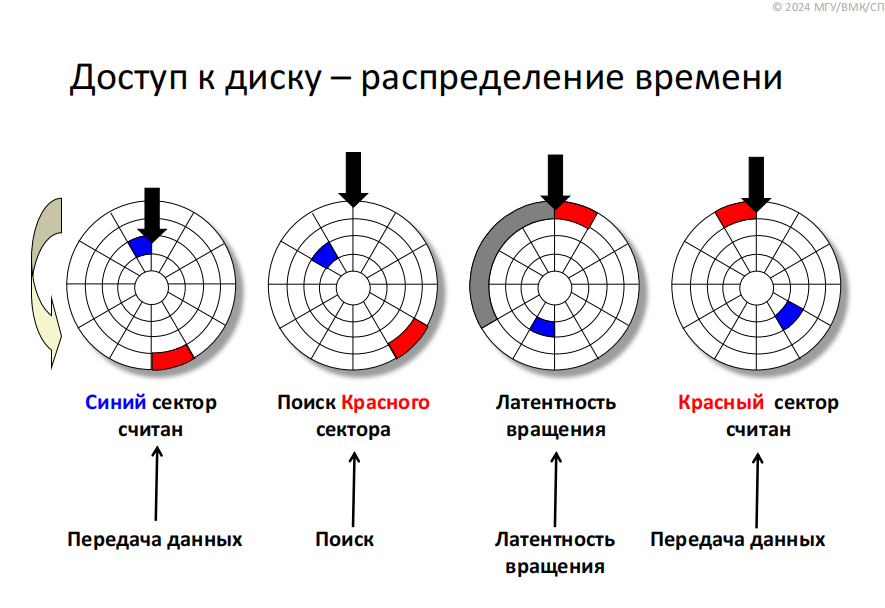
\includegraphics[width=0.7\linewidth]{image1.png}
\end{figure}
\\
Тогда время необходимое на считывание одного произвольно расположенного сектора вычисляется по формуле:\\
$T_\text{доступа}=T_\text{ср. поиск}+T_\text{ср. вращения}+T_\text{ср. передача}$\\
1) $T_\text{ср. поиск}$ (время поиска) - время, необходимое, что бы переместить считывающую головку на нужную дорожку (цилиндр).\\
2) $T_\text{ср. вращения}$ (латентность вращения) - время ожидания момента, когда первый бит нужного сектора достигнет считывающей головки.\\
Вычисляется по формуле:\\
$T_\text{ср. вращения}=\frac{1}{2} * (60/v_\text{вращения})$ (если $v_\text{вращения}$ задана в RPM).\\
3)$T_\text{ср. передача}$ (время передачи) - время чтения содержимого сектора.\\
Вычисляется по формуле:\\
$T_\text{ср. передача} = \frac{1}{\text{ср. кол-во секторов на дорожке}} * 2T_\text{ср. вращения}$\\
$2T_\text{ср. вращения}$ - это время, за которое диск делает полный оборот.\\

\textbf{Произвольное размещение данных} - каждый блок данных находится в произвольном месте диска, поэтому для чтения каждого блока необходимо каждый раз выполнять поиск дорожки и ожидать момента когда первый бит нужного блока достигнет считывающей головки.\\

\textbf{Наилучшее размещение данных} - блоки данных расположены подряд на одной дорожке (если есть несколько поверхностей, то на дорожках соответствующих одному цилиндру). Время поиска и латентность вращения тратятся только в начале считывания и при переходе от одного цилиндра к другому.\\

\subsubsection{Решение}
1. Файл размером 9 МиБ разделен на логические блоки по 4096 байт.\\
9 МиБ = $9*2^{20}$ байт\footnote{МиБ (мибибайты) - степень 2 $= 2^{20}$, тогда как Мб (мегабайты) - степень 10 $= 10^6$}. Значит всего блоков $9*2^{20}/4096=2304$.\\

\textbf{Пункт А):}\\
Среднее число секторов на дорожке: 512.\\
Размер сектора = размер блока.\\
Значит на дорожке можно разместить 512 блоков.\\
Число поверхностей: 4.\\
Значит в одном цилиндре 4 дорожки.\\
Поэтому можем считать подряд $512 * 4 = 2048$ блока. Останется еще 256 блока. Их считаем из следующего цилиндра.\\

Итого:\\
1) Находим нужный цилиндр ($T_\text{ср. поиск}$)\\
2) Ждем латентность вращения ($T_\text{ср. вращения}$)\\
3) Считываем подряд 2048 блоков ($2048 * T_\text{ср. передача}$)\\
4) Находим другой цилиндр  ($T_\text{ср. поиск}$)\\
5) Ждем латентность вращения ($T_\text{ср. вращения}$)\\
6) Считываем подряд 256 блоков ($256 * T_\text{ср. передача}$)\\

Далее, $T_\text{ср. поиск} = 2$ мс. по условию.\\
$T_\text{ср. вращения}=\frac{1}{2} * (60/v_\text{вращения}) = \frac{1}{2} * (60/15000) = 0,002$ с. $= 2$ мс.\\

$T_\text{ср. передача} = \frac{1}{\text{ср. кол-во секторов на дорожке}} * 2T_\text{ср. вращения} = \frac{1}{512} * 2 * 2$ мс.\\

Результат: $2 * T_\text{ср. поиск} + 2 * T_\text{ср. вращения} + 2304 * T_\text{ср. передача} = 2 * 2 + 2 * 2 + 2304 * \frac{1}{512} * 2 * 2 = 26$ мс.\\

\textbf{Пункт Б):}\\
Мы уже знаем, что:
\begin{itemize}
\item всего блоков 2304
\item $T_\text{ср. поиск} = 2$ мс
\item $T_\text{ср. вращения} = 2$ мс
\item $T_\text{ср. передача} =\frac{1}{512} * 2 * 2$ мс
\end{itemize}
Если размещение произвольное, то перед считыванием каждого блока необходимо потратить $T_\text{ср. поиск}$ и $T_\text{ср. вращения}$. Значит, результат: $2304 * (T_\text{ср. поиск} + T_\text{ср. вращения} + T_\text{ср. передача} = 2304 * (2 + 2 + \frac{1}{512} * 2 * 2) = 9234$ мс.\\

\textbf{Ответ:}\\
А) 26 мс.\\
Б) 9234 мс.
\newpage
\end{document}